\section{Baseline Ben-Porath Model} \label{section:baseline}
\noindent The first and very basic model builds on the following five assumptions: (i) a single representative agent; (ii) perfect capital markets; (iii) no non-market benefits of human capital; (iv) fixed labor supply; (v) constant depreciation of human capital stock, $\sigma$. Let $T$ define a time horizon. This model is known as the Ben-Porath model.\\
\indent For each $t \in T$, $H$ denotes human capital, $I \in [0,1]$ investment time, $D$ market goods that serve as inputs to the production function, and $F$ a strictly concave production function in two normal inputs. The law of motion for human capital is
\begin{equation}
\dot{H(t)} = F \left( I(t) H(t), D(t) \right) - \sigma H(t) \label{eq:lawh}
\end{equation}
and embeds a neutrality assumption. Namely, the current stock of human capital at time $t$, $H(t)$, and the investment time at time $t$, $I(t)$, appear as a single argument in a multiplicative fashion in the flow production of human capital. At each point of time, the current stock and the rental rate of human capital, $R$, define potential earnings
\begin{equation}
Y(t) = R H(t).
\end{equation}

\indent In general, observed earnings and potential earnings differ by two terms, foregone earnings and direct market goods costs. Let $P_{D}$ be the price of markets and define observed earnings, $E(t)$ as
\begin{equation}
E(t) = R H(t) -  R I(t) H(t) - P_{D} D(t) \label{eq:earnings}
\end{equation}
where $R I(t) H(t)$ are foregone earnings and $ P_{D} D(t) $ are direct goods costs. This expression clarifies that $I(t)$ is the fraction of time devoted to investment in each period of time. In particular, the individual occupies a fraction $I(t)$ of her human capital stock to produce a human capital flow.\\ 
\indent The individual chooses $D(t)$ and $I(t)$ to maximize her lifetime earnings stream given an initial level of human capital, $H(0) = H_{0}$ and subject to the law of motion of human capital, \eqref{eq:lawh}.\\
\indent The \textit{current value Hamiltonian} associated to the individual's problem is
\begin{equation}
\mathcal{H} (\cdot) = e^{-rt} \left[ R H(t) -  R I(t) H(t) - P_{D} D(t) \right] + \mu_{t} \dot{H(t)} 
\end{equation}
where $\mu(t)$ defines the shadow price of human capital. For a strictly concave function $F(\cdot)$ the necessary and sufficient conditions for optimality are
\begin{eqnarray}
\frac{\partial \mathcal{H} (\cdot)}{\partial I(t)} = 0 &\Leftrightarrow& e^{-rt}R = \mu(t) F_{I(t)H(t)} \label{eq:focinvestment} \\
\frac{\partial \mathcal{H} (\cdot)}{\partial D(t)} = 0 &\Leftrightarrow& e^{-rt}R I(t) = \mu(t) F_{D(t)} \label{eq:focgoods} \\
\frac{\partial \mathcal{H} (\cdot)}{\partial H(t)} = - \dot{\mu(t)} &\Leftrightarrow& e^{-rt} R \left( 1 - I (t) \right) + \mu(t) \left(  F_{I(t)H(t)} - \sigma \right) = - \dot{\mu(t)} \label{eq:focstock} \\ 
\frac{\partial \mathcal{H} (\cdot)}{\partial \mu(t)} = \dot{H(t)} &\Leftrightarrow& \dot{H(t)} = F \left( I(t) H(t), D(t) \right) - \sigma D(t) \label{eq:focmotion} \\
\text{Transversality} &:& \lim_{t \rightarrow T} \mu(t) H(t) = 0 \label{eq:foctransversality}
\end{eqnarray}
where $F_{j} \equiv \frac{\partial F \left( I(t), D(t) \right) }{\partial j}$ for $j = D(t), I(t) H(t)$. Combine \eqref{eq:focinvestment} and \eqref{eq:focstock} to get 
\begin{equation}
\dot{\mu(t)} = - e^{-rt} R + \mu(t) \sigma \label{eq:focinvstockcombine}.
\end{equation}

\noindent Let $g(t) \equiv \mu(t) e^{rt}$ and note that $\dot{g(t)} = \dot{\mu(t)} e^{rt} + r \mu(t) e ^{rt}$. Use \eqref{eq:focinvstockcombine} to obtain 
\begin{equation}
\dot{g(t)} = (\sigma + r ) g(t) - R \label{eq:grossdep}.
\end{equation}

\indent $g(t)$ has fundamental importance to this problem because it is a discount factor that adjusts for exponential depreciation of gross investment and enables to write the individual's problem in a more intuitive way. In particular, note that \eqref{eq:foctransversality} implies that $\mu(T) = 0 $ and, therefore, $g(T) = 0$.\footnote{Note that $H(T) > 0$ because otherwise the individual losses the possibility to earn in the last period.} Thus, it is possible to solve \eqref{eq:grossdep} and obtain
\begin{equation}
g(t) = \frac{R}{\sigma + r} \left[ 1 - e^{(\sigma + r)(t - T)} \right].
\end{equation}

\indent Importantly, for an interior solution, this enables to analyze the problem in $t$ and obtain all the features of the investment dynamics and human capital accumulation. In particular, the problem of the agent is to maximize her discounted gross flow of human capital less her costs (foregone earnings plus market goods costs) 
\begin{equation}
\max_{I(t), D(t)} \left[ g(t) F(I(t) H(t), D(t)) - P_{D} D(t) - R I (t) H(t) \right]
\end{equation}
for which the first order conditions are
\begin{eqnarray}
g(t) F_{I(t)H(t)} H(t) &=& R H (t) \nonumber \\
g(t) F_{D(t)} H(t) &=& P_{D} \label{eq:newfocs}. 
\end{eqnarray}

The system in \eqref{eq:newfocs} results on a system of two equations and two unknowns that solves for the Marshallian demands of $I(t)H(t)$ and $D(t)$. Input normality together with the fact that $\dot{g(t)} < 0$ imply that the both Marshallian demands are decreasing overtime, which is intuitive because the agent faces a finite horizon problem.\footnote{Need to think why $g(t)$ is decreasing over time.} This provides the necessary arguments to analyze earnings dynamics in this first simple model.
\subsection{Earnings Dynamics}
\subsubsection{No Human Capital Depreciation}
Suppose that there is no human capital depreciation. Take the definition of earnings, \eqref{eq:earnings}, and note that
\begin{eqnarray}
\dot{E(t)} &=& R \dot{H(t)} - R \dot{I(t)H(t)} - P_{D} \dot{D(t)} \nonumber \\
           &=& R F \left( I(t) H(t), D(t) \right) - R \dot{I(t)H(t)} - P_{D} \dot{D(t)} \nonumber \\     
           &>& 0 
\end{eqnarray}

\noindent where the second equality follows from the law of motion for human capital when $\sigma = 0$.\footnote{Clear up the intuition of this result.}\\
\indent In the case of human capital depreciation earnings are not necessarily monotonic because $\dot{E(t)} = R F \left( I(t) H(t), D(t) \right) - R \sigma H(t) - R \dot{I(t)H(t)} - P_{D} \dot{D(t)}$ and $| R \sigma H(t) | $ may be big enough to make $\dot{E(t)}$ over some periods.
\subsubsection{No Depreciation and the Cobb-Douglas Production Function for Human Capital}

\noindent The simplest version of this model occurs when $\sigma = 0$ and $F(I(t) H(t), D(t))$ is a Cobb-Douglas production function. \citet{ben1967production} shows that in this case $\dot{E(t)} > 0, \ddot{E(t)} < 0$. This is, earnings increase at a decreasing rate over the life cycle.\\

\subsection{Earnings Growth Dynamics} \label{section:egdyn}
It is of relevance to understand how earnings behave in cases that are more general relative to Cobb-Douglas. For that sake assume that $F_{D(t)} = 0 $, i.e. assume away $D(t)$ and therefore let $F(\cdot)$ take a single argument, $I(t) H(t)$. The first order condition for investment becomes
\begin{equation}
g(t) F'(I(t) H(t)) = R
\end{equation}
and we can differentiate with respect to $t$ and get
\begin{eqnarray}
\dot{g(t)} F'(I(t) H(t)) + g(t) F''(I(t) H(t)) \dot{I(t) H(t)} &=& 0 \nonumber \\
&\Leftrightarrow& \nonumber \\
\dot{I(t) H(t)} &=& - \left( \frac{\dot{g(t)}}{g(t)} \right) \left[ \frac{F'}{F''}\right] \label{eq:itdot}.
\end{eqnarray}
\noindent Moreover, drop the argument $t$ to shorten notation, and note that
\begin{eqnarray}
\ddot{IH} = - \left[ \frac{\ddot{g}}{g} - \left( \frac{\dot{g}}{g} \right)^2 \right] \frac{F'}{F''} + \left( \frac{\dot{g}}{g} \right)^2 \left[ 1 - \frac{F'F'''}{{F''}^2} \right] \left[ \frac{F'}{F''} \right]  
\end{eqnarray}  
where we substitute in $\eqref{eq:itdot}$.\\
\indent Without lost of generality assume that $R = 1$ and note that
\begin{eqnarray}
\dot{E} &=& F(IH) - \dot{IH} - \sigma H \nonumber \\
\ddot{E} &=& F'(IH) \dot{IH} - \ddot{IH} - \sigma \dot{H} \nonumber \\
&=& \frac{1}{g} \dot{IH} - \ddot{IH} - \sigma \dot{H}.
\end{eqnarray}
Now, let $\sigma = 0$ and from \eqref{eq:grossdep} obtain $\frac{\ddot{g}}{g} = r \frac{\dot{g}}{g}$. Thus,
\begin{eqnarray}
\ddot{E} &=& - \frac{\dot{g}}{g} \frac{F'}{F''} \left[ \frac{1}{g} - \frac{\dot{g}}{g} \left( 1 - \frac{F'F'''}{{F''}^2} \right) \right] + \left[ r \frac{\dot{g}}{g} - \left( \frac{\dot{g}}{g} \right)^2 \right] \frac{F'}{F''} \nonumber \\
&=& - \frac{\dot{g}}{g} \frac{F'}{F''} \left[ \frac{1}{g} - \frac{\dot{g}}{g} \left( 1 - \frac{F'F'''}{{F''}^2} \right) - \frac{gr - \dot{g}}{g} \right] \nonumber \\
&=& - \frac{\dot{g}}{g} \frac{F'}{F''} \left[ \frac{1}{g} - \frac{\dot{g}}{g} \left( 1 - \frac{F'F'''}{{F''}^2} \right) - \frac{1}{g} \right] \nonumber \\
&=& - \left( \frac{\dot{g}}{g} \right)^2 \frac{F'}{F''} \left( 1 - \frac{F'F'''}{{F''}^2} \right)
\end{eqnarray}

\noindent where the third equality uses \eqref{eq:grossdep}, i.e. $gr - \dot{g} = 1$. F is strictly concave and therefore $-\left( \frac{\dot{g}}{g} \right)^2 \frac{F'}{F''} > 0$. The sign of $\eta \equiv \left( 1 - \frac{F'F'''}{{F''}^2} \right)$ depends on $F'''$. A sufficient condition for $\dot{E}$ to be concave is $\eta < 0$.
\begin{example} (Human Capital Production Functions and Earnings Concavity)
\begin{itemize}
\item Power Production Function 1 : consider the case of $F(x) = \frac{Ax^{\alpha}}{\alpha}$ for $ - \infty < \alpha < 1, A > 0$. Then, $\eta = \frac{1}{\alpha - 1} < 0$. Under this specification the earnings function is strictly concave with respect to time.
\item Power Production Function 2 : consider the case of $F(x) = a - b x ^ {- \alpha}$ for $ - 1 < \alpha < \infty, a,b,c > 0$. Then, $\eta = \frac{-1}{\alpha + 1} < 0$. Under this specification the earnings function is strictly concave with respect to time.
\item Quadratic Production Function: any quadratic production function has $F''' = 0$ and does not induce concavity of earnings with respect to time. 
\end{itemize}
\noindent Importantly, all this examples consider no depreciation of human capital, $\sigma = 0$. 
\end{example} 

\subsection{Specialization Period}
A period of specialization happens when the agent devotes his complete time to produce a flow of human capital, i.e. when $I(t) = 1$ for $t \in [ \underline{t}, \bar{t}]$. In order to illustrate assume away $D(t)$ so that $F_{D(t)} = 0$ and $\sigma = 0$, i.e. no human capital depreciation. First note that the marginal returns to investment decline as the stock of human capital grows and overtime. Concavity of $F(\cdot)$ causes the first implication while $\dot{g} < 0$ causes the second. Then, there is at most one period of specialization at the beginning of the time horizon, if it happens: $[0,t^*]$. This is what \citet{ben1967production} calls schooling period.\\
\indent Four conditions hold in the specialization period
\begin{eqnarray}
F'(H(t))g(t) &>& R \nonumber \\
F'(H(t^*))g(t^*) &=& R \nonumber \\
I(t^*) &=& 1 \nonumber \\
H(t^*) &=& \int \limits _{0} ^{t^*} F (H(\tau)) d\tau + H_{0} \label{eq:humantstar}
\end{eqnarray} 
\noindent where $H(t^*)$ is the human capital stock accumulated up to time $t^*$, the sum over the period $[0,t^*]$ plus the initial stock.\\
\indent Given that $R$ is fixed at $1$, any decrease in $g(t)$ lowers $t^*$ because it lowers the discount to gross investment in human capital. For example, relatively high $r$ implies relatively low $t^*$ because the individual is relatively present oriented. Also, from the \eqref{eq:humantstar}, note that a high value of $t^*$ implies lower value for $t^*$ because it takes less time to obtain $H(t^*)$.\footnote{A more realistic model, perhaps, makes $R$ depend on human capital so that more able individuals find it cheaper to invest in human capital. However, they also have higher foregone earnings and we cannot say without deeper analysis how $t^*$ behaves in such a case.} If $\sigma > 0 $ the the same conditions characterize specialization. However, the there may be more than one specialization period because, under some scenarios, a high value of $\sigma$ may knock off capital such that investment cycles are optimal. We stay away from such scenarios and keep $\sigma = 0$ in what follows.
\begin{example} (No Depreciation and the Cobb-Douglas Production Function for Human Capital: Initial Human Capital and the Specialization Period) \label{example:ndcdexample}
In this case $\dot{H} = A \left(IH \right)^\alpha$ where $0 < \alpha < 1, A>0$. As argued above, specialization happens in the period $[0,t^*]$. Thus
\begin{eqnarray}
	\alpha A \left( H(0) \right) ^{\alpha - 1 }g(0) &>& R \nonumber \\
	&\Leftrightarrow& \nonumber \\
	H(0) &<& \left[ \frac{R}{g(0)\alpha A} \right]^{\frac{1}{\alpha-1}} \label{eq:h0forspe}.
\end{eqnarray}
\indent As the conditions in \eqref{eq:humantstar} establish, the time spent in specialization is a decreasing function of $H(0)$. In this example, actually, the initial human capital needs to be below certain threshold in order for the individual to specialize during one period. 
\end{example}

\begin{example} (Infinite Horizon)
In the setting of Exercise \ref{example:ndcdexample} and if the horizon of the problem is infinite: $H(0) < \left( \frac{\alpha A}{r} \right) ^{\frac{1}{1 - \alpha}}$ because $g(t) = \frac{R}{r}$.
\end{example}

\begin{example} (No Depreciation and the Cobb-Douglas Production Function for Human Capital: the Specialization Period)
In the period of specialization $I(t) = 1$. Then,
\begin{equation}
\dot{H} = A \left( H \right)^{\alpha} \label{eq:humandiff}.
\end{equation}
The general solution for \eqref{eq:humandiff} is
\begin{equation}
H(t) = \left[ (1 - \alpha)(At + K) \right]^{\frac{1}{1-\alpha}}
\end{equation}
for some constant $K$. Given an initial condition $H(0) = H_{0}$, $K = \frac{H_{0}^{1-\alpha}}{1-\alpha}$ and
\begin{equation}
H(t) = \left[ (1 - \alpha)At + H_{0}^{1-\alpha} \right]^{\frac{1}{1-\alpha}} \label{eq:hbeforetstar}.
\end{equation}
At the end of the specialization period, as established in \eqref{eq:humantstar}:
\begin{equation}
\alpha g(t^*) A \left( H(t^*) \right)^{\alpha - 1} = R.
\end{equation}
If $T \rightarrow \infty$, $g(t) = \frac{R}{r}$ and
\begin{equation}
t^* = - \frac{H_{0}^{1 - \alpha}}{A(1 - \alpha)} + \frac{\alpha}{1 - \alpha}\frac{1}{r}. \label{eq:tstar}
\end{equation}

\indent \eqref{eq:tstar} provides some intuitive results: (i) an individual with relatively high initial human capital specializes during a relatively shorter period: $\frac{\partial t^*}{\partial       H_{0}} < 0$; (ii) a relatively abler individual specializes during relatively longer period: $\frac{\partial t^*}{\partial A} > 0$; a relatively impatient individual specializes for a relatively shorter period: $\frac{\partial t^*}{\partial r} < 0$.
\end{example}

\begin{example} (No Depreciation and the Cobb-Douglas Production for Human Capital: Post-experience Earnings)
Let $\tau = t - t^*$ define the post-school work experience and write post-school earnings as follows:
\begin{equation}
E(\tau) = R \int \limits _{0} ^{\tau} \dot{H( l + t^*)}d l + R H(t^*) - RIH(\tau + t^*).
\end{equation}
Now, from \eqref{eq:humantstar} the following equality holds:
\begin{eqnarray}
\alpha g(t) A \left( IH(t) \right)^{\alpha - 1} &=& R \nonumber \\
&\Leftrightarrow& \nonumber \\
IH(t) &=& \left[ \frac{\alpha g(t) A}{R} \right]^{\frac{1}{1-\alpha}} \label{eq:itcobb}
\end{eqnarray}
Combining \eqref{eq:itcobb} and the law of motion for human capital:
\begin{equation}
\dot{H} = A \left[ \frac{\alpha g(t) A}{R} \right]^{\frac{\alpha}{1-\alpha}} \label{eq:hdot}.
\end{equation}
Then,
\begin{equation}
E(\tau) = R \int \limits _{0} ^{\tau} A \left[ \frac{\alpha g(l + t^*) A}{R} \right]^{\frac{\alpha}{1-\alpha}} dl + RH(t^*) - R \left[ \frac{\alpha g \left( \tau + t^* \right) A}{r} \right]^{\frac{1}{1-\alpha}} \label{equation:postearnings}
\end{equation}
and if $T \rightarrow \infty$
\begin{equation}
E(\tau) = RA \left[ \frac{\alpha A}{R} \right]^{\frac{\alpha}{1-\alpha}} \tau.
\end{equation}

\begin{center}
\begin{figure}[H]
\caption{Earnings and Experience, Cobb Douglas Technology and No Depreciation}
\centering
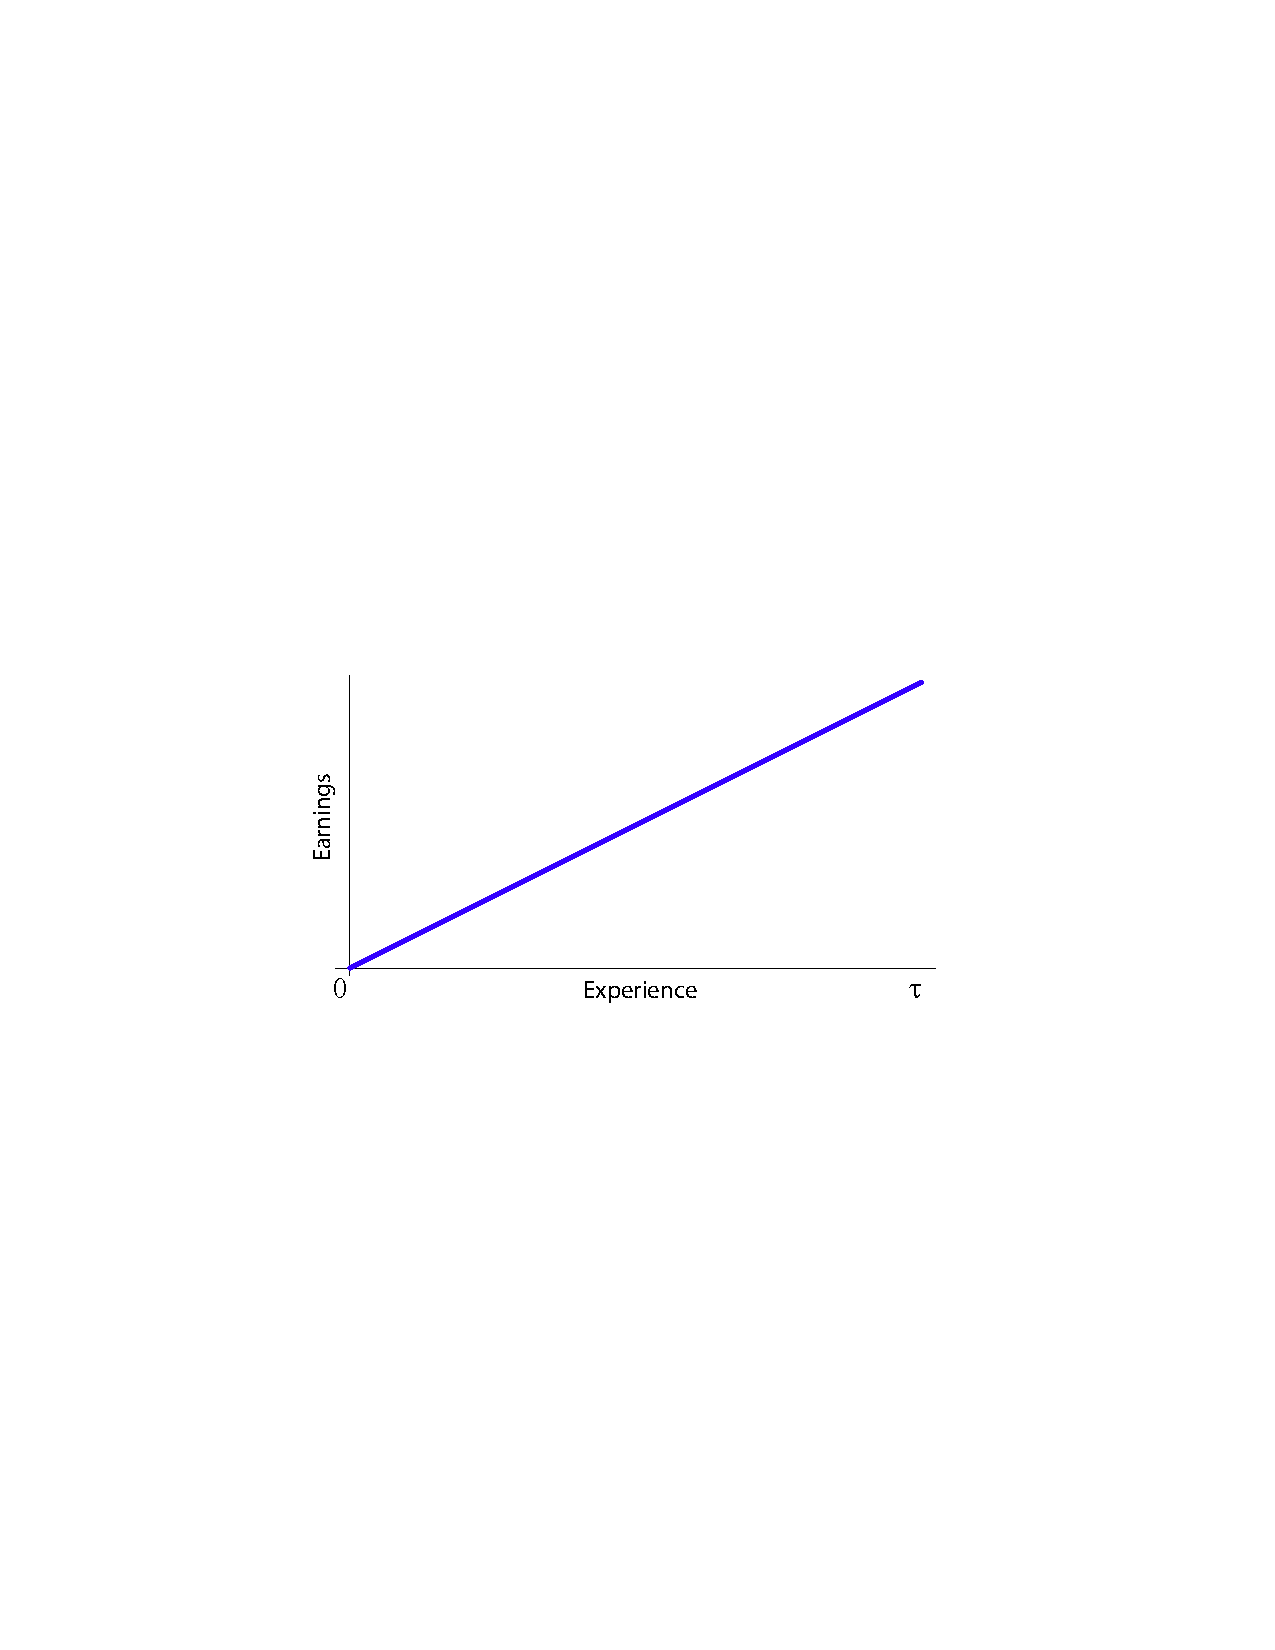
\includegraphics[width=3.5in, height=1.5in]{Figures/fig-earnings-experience.pdf}
\floatfoot{\begin{small}
Note:
\end{small}}
\end{figure}
\end{center}

\end{example}

\subsection{The Baseline Model Dynamics under the Cobb-Douglas Specification: a Summary}
This section summarizes the dynamics of the main variables in the baseline model when there is no depreciation and market goods are ruled out as inputs for the production of human capital investment. We assume that the horizon is infinite to simplify the algebra but it is important to remark that the qualitative properties of the results remain unchanged under finite horizon. At the end we show simulations that illustrate how the variables of interest behave under various parametrizations. 

\subsubsection{Human Capital}
\begin{itemize}
\item At $t = 0$ an initial condition is given.
\item At $0 < t < t^*$ the system \eqref{eq:humantstar} provides the conditions that human capital satisfies and its expression is given by \eqref{eq:hbeforetstar}.
\item At $t = t^*$ \eqref{eq:hbeforetstar} is still a valid expression for human capital. To obtain the exact quantity it suffices to evaluate the expression for $t^*$, \eqref{eq:tstar}, into \eqref{eq:hbeforetstar}.
\item At $ t > t^* $ \eqref{eq:humantstar} and the expression for $\dot{H}$, \eqref{eq:hdot}, provide the expression for human capital.
\end{itemize}

Then,\footnote{There is a mistake in the definition of this function in the notes}

\begin{eqnarray}
H(t) =
\begin{cases}
H_{0} & t = 0 \\
\left[ (1 - \alpha)At + H_{0}^{1-\alpha} \right]^{\frac{1}{1-\alpha}} , & 0 < t < t^* \\
\left[ \frac{\alpha A}{r} \right]^{\frac{1}{1 - \alpha}}, & t = t^* \\
\left[ \frac{\alpha A}{r} \right]^{\frac{ \alpha }{1 - \alpha}} \left( t - t^* \right) + \left[ \frac{\alpha A}{r} \right]^{\frac{1}{1 - \alpha}} , & t > t^*. \label{eq:humancapall}
\end{cases}
\end{eqnarray}

\subsubsection{Investment}
We focus on the case in which there is an specialization period, i.e. the case in which \eqref{eq:h0forspe} holds. The combination of \eqref{eq:itcobb} and \eqref{eq:humancapall} gives the following

\begin{eqnarray}
I(t) =
\begin{cases}
1, & t = 0 \\
1, & 0 < t < t^* \\
1, & t = t^* \\
\frac{\left[ \frac{\alpha A}{r} \right]^{\frac{1}{1 - \alpha}}}{\left[ \frac{\alpha A}{r} \right]^{\frac{ \alpha }{1 - \alpha}} \left( t - t^* \right) + \left[ \frac{\alpha A}{r} \right]^{\frac{1}{1 - \alpha}}}, & t > t^*. \label{eq:investall}
\end{cases}
\end{eqnarray}

\subsection{Earnings}
For the case of earnings we also on the case in which there is an specialization period, i.e. the case in which \eqref{eq:h0forspe} holds. Thus, \eqref{eq:earnings}, \eqref{eq:humancapall}, \eqref{eq:investall} define earnings as follows

\begin{eqnarray}
E(t) =
\begin{cases}
0, & t = 0 \\
0, & 0 < t < t^* \\
0, & t = t^* \\
RA \left[ \frac{\alpha A}{r} \right]^{\frac{\alpha}{1 - \alpha}} \left( t - t^* \right) , & t > t^*. \label{eq:earnsall}
\end{cases}
\end{eqnarray}

\subsubsection{Graphical Analysis}
We now produce simulations to illustrate the comparative statics of the model. In all of them we set $R=1$.

\begin{figure}[H]
     \begin{center}
    			\caption{Dynamics for $A = 3, r = .05, H_{0} = 1$ \\ $\alpha = .3$ (dotted); $\alpha = .4$ (dashed); $\alpha = .5$ (solid) }
        \subfigure[Human Capital Investment]{
            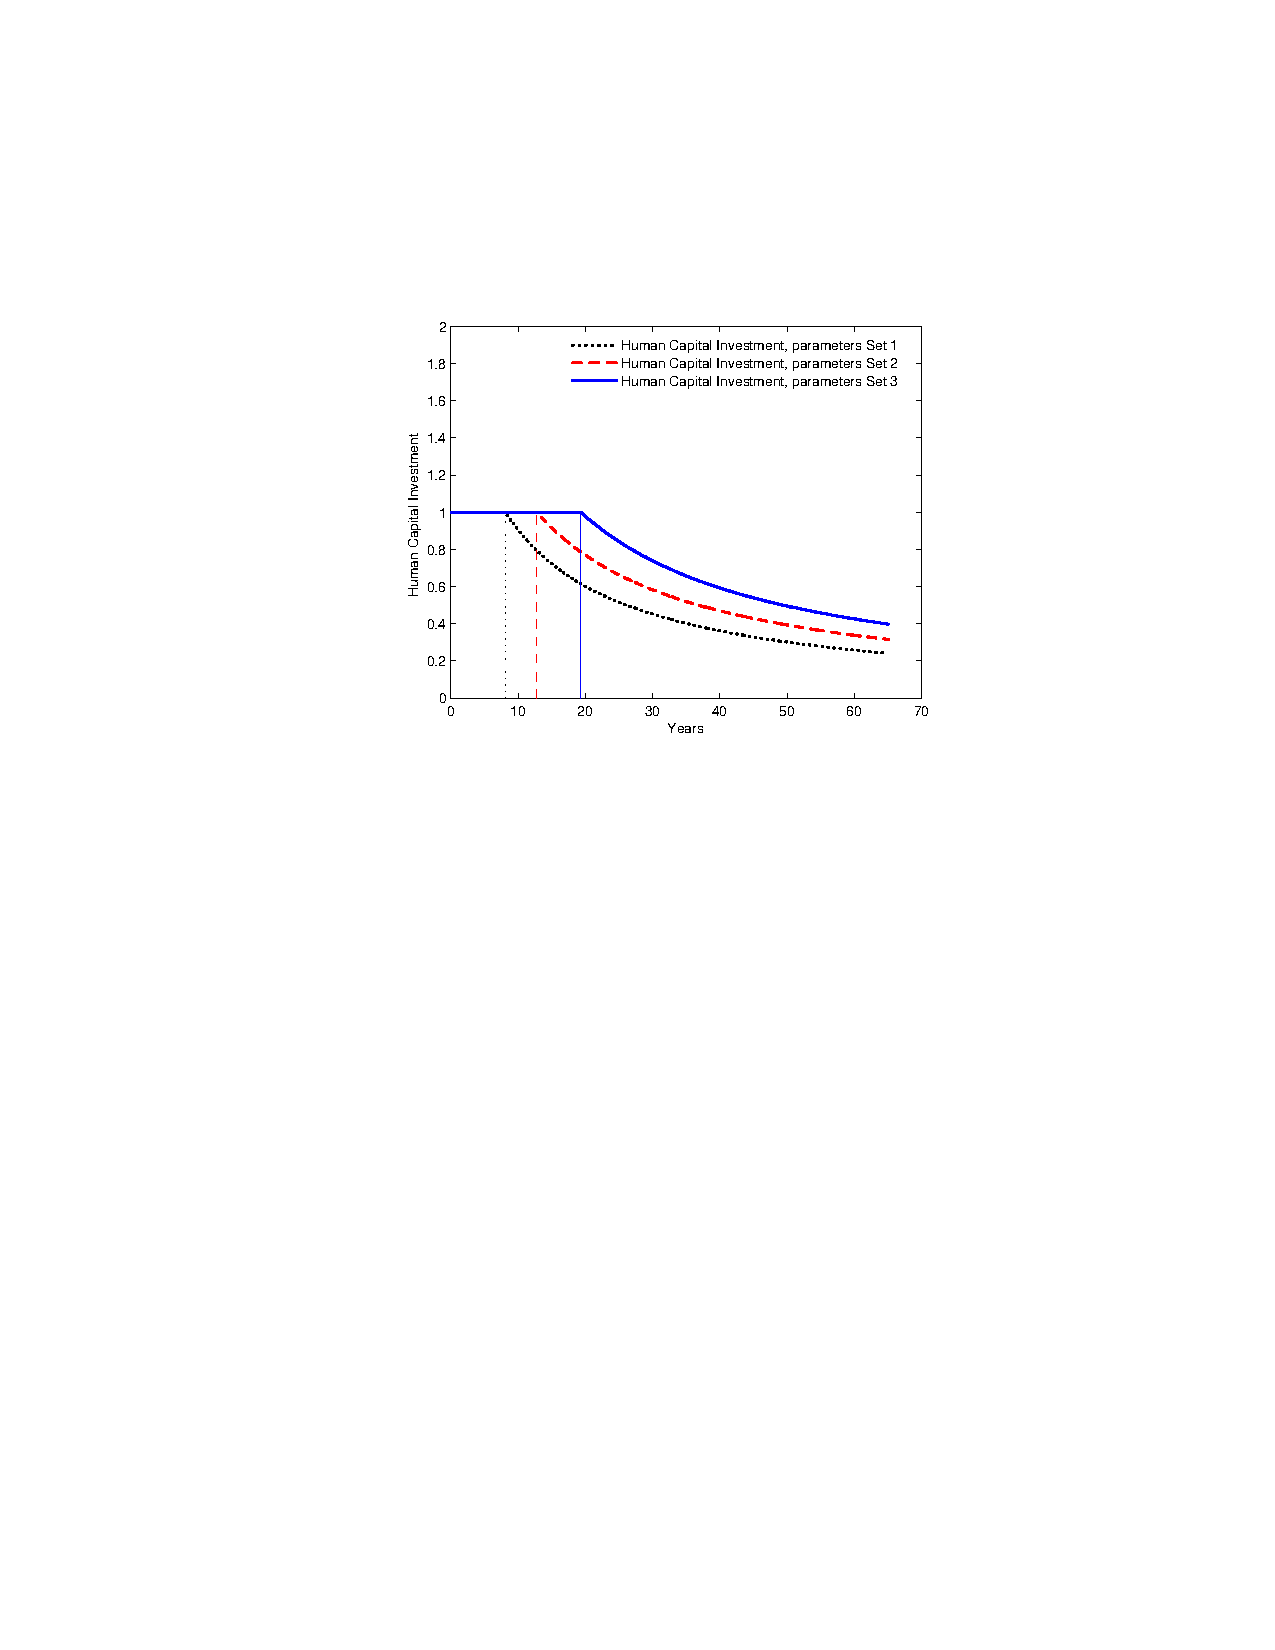
\includegraphics[width=2.2in, height=2.2in]{Figures/fig-hc-earn-series-02.pdf}
        }\\
        \subfigure[Human Capital Stock]{
            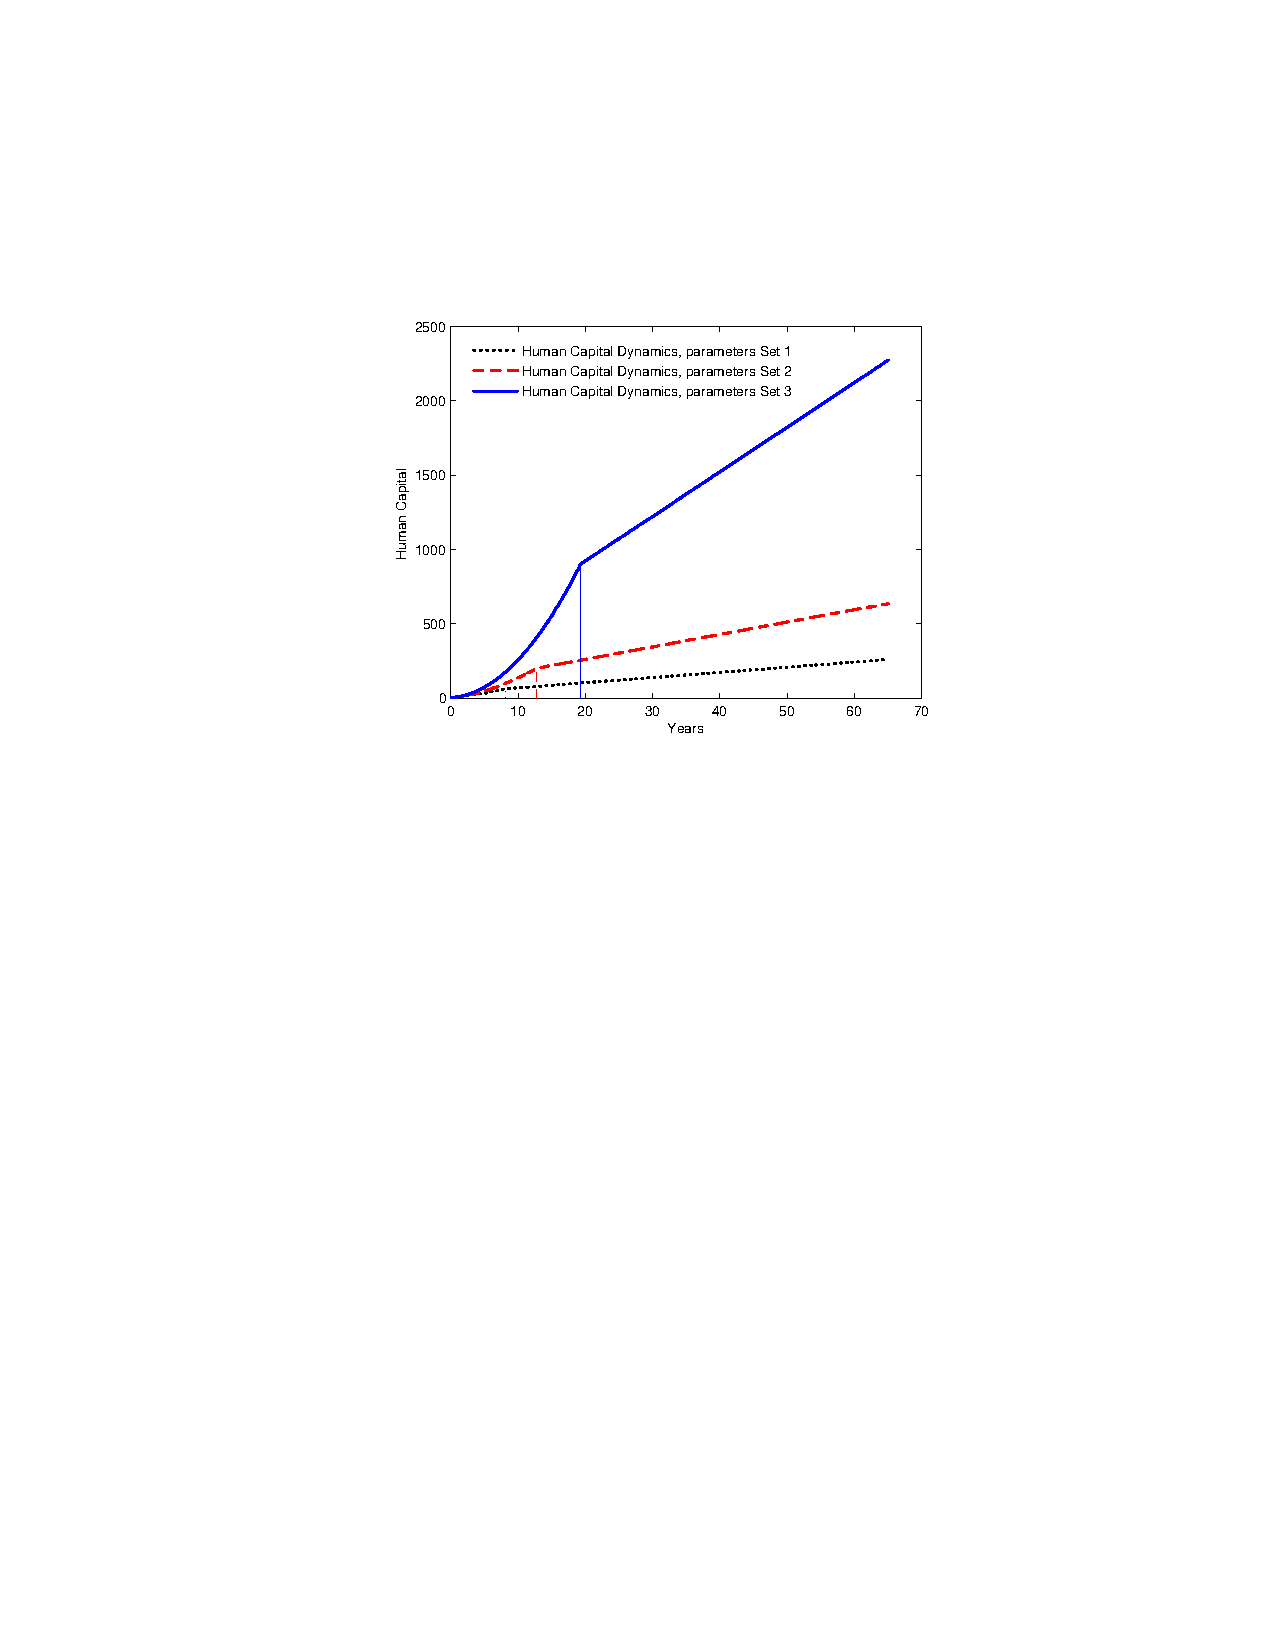
\includegraphics[width=2.2in, height=2.2in]{Figures/fig-hc-earn-series-01.pdf}
        }\\
        \subfigure[Earnings]{%
            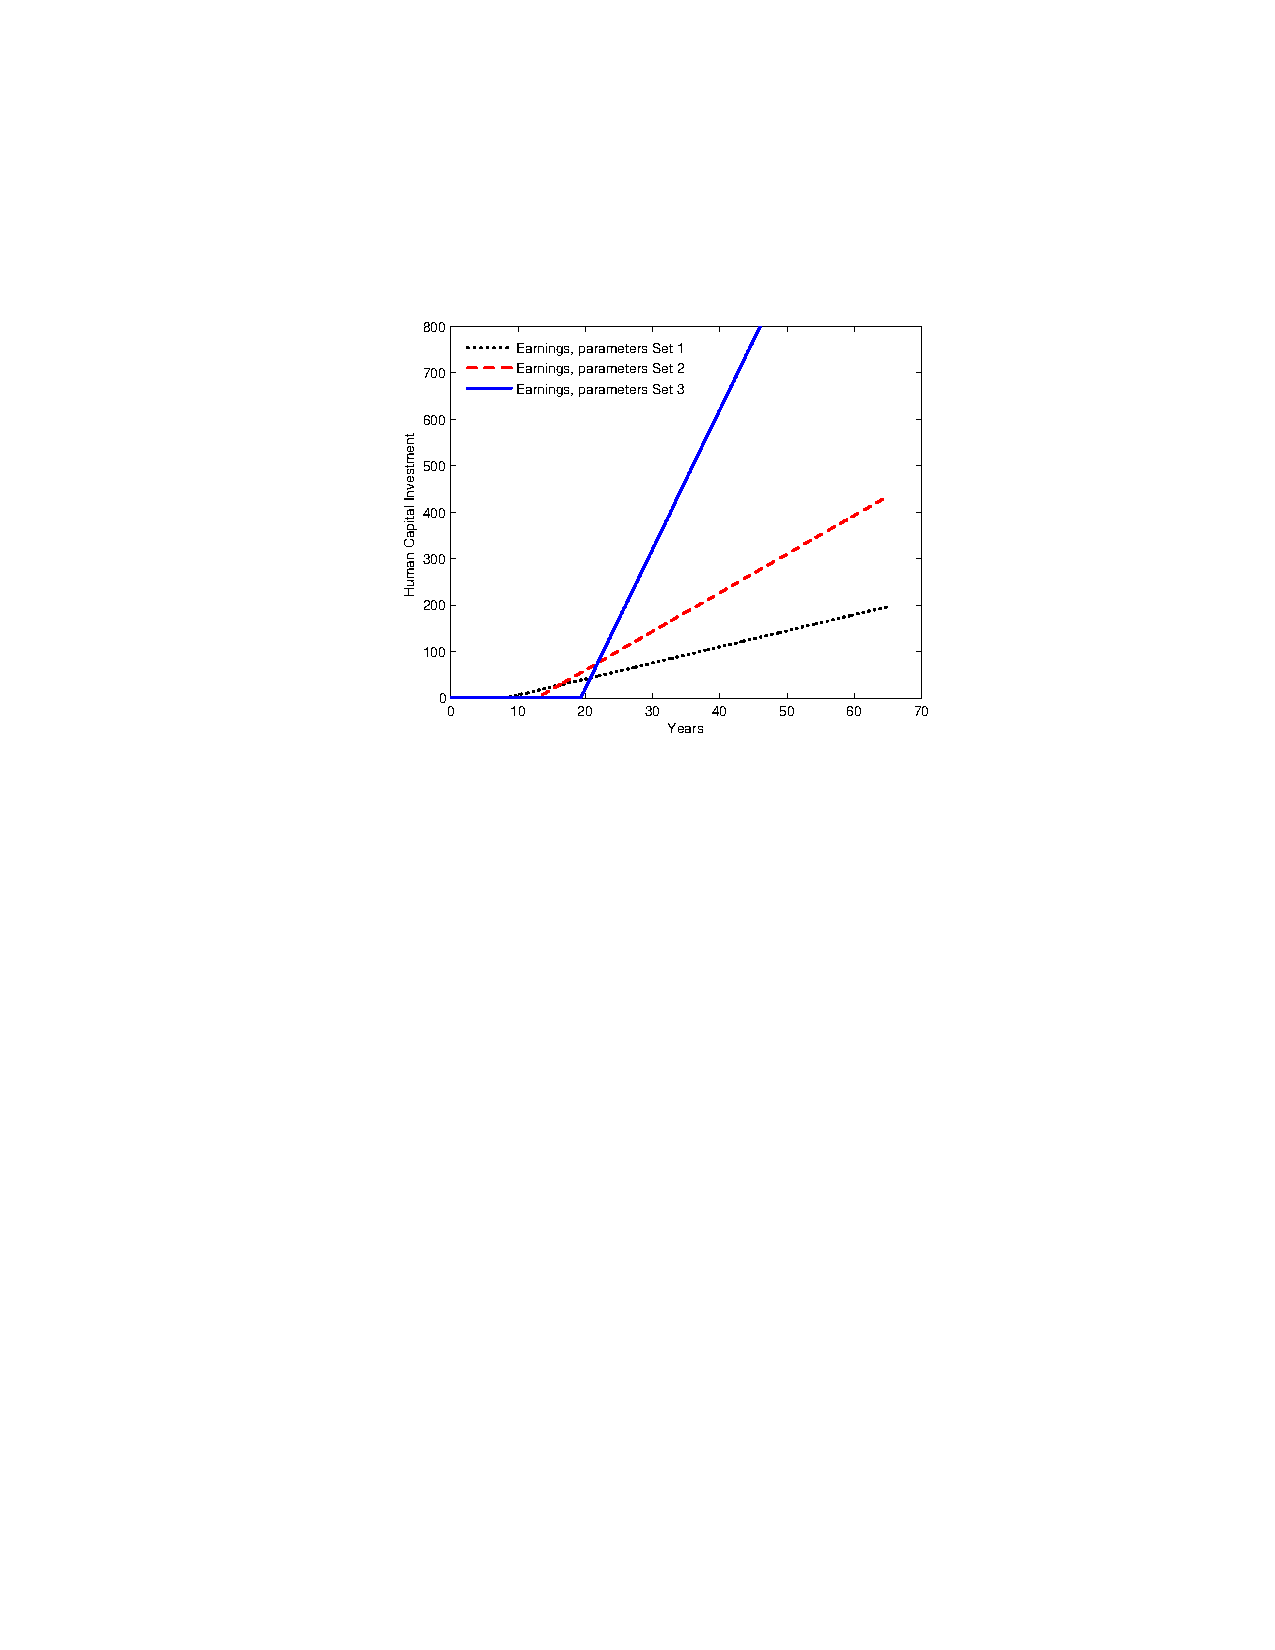
\includegraphics[width=2.2in, height=2.2in]{Figures/fig-hc-earn-series-03.pdf}
        }
    \end{center}
\end{figure}

\begin{figure}[H]
     \begin{center}
    			\caption{Dynamics for $A = 3, \alpha = .5, H_{0} = 1$ \\ $r = .04$ (dotted); $r = .05$ (dashed); $r = .06$ (solid) }
        \subfigure[Human Capital Investment]{
            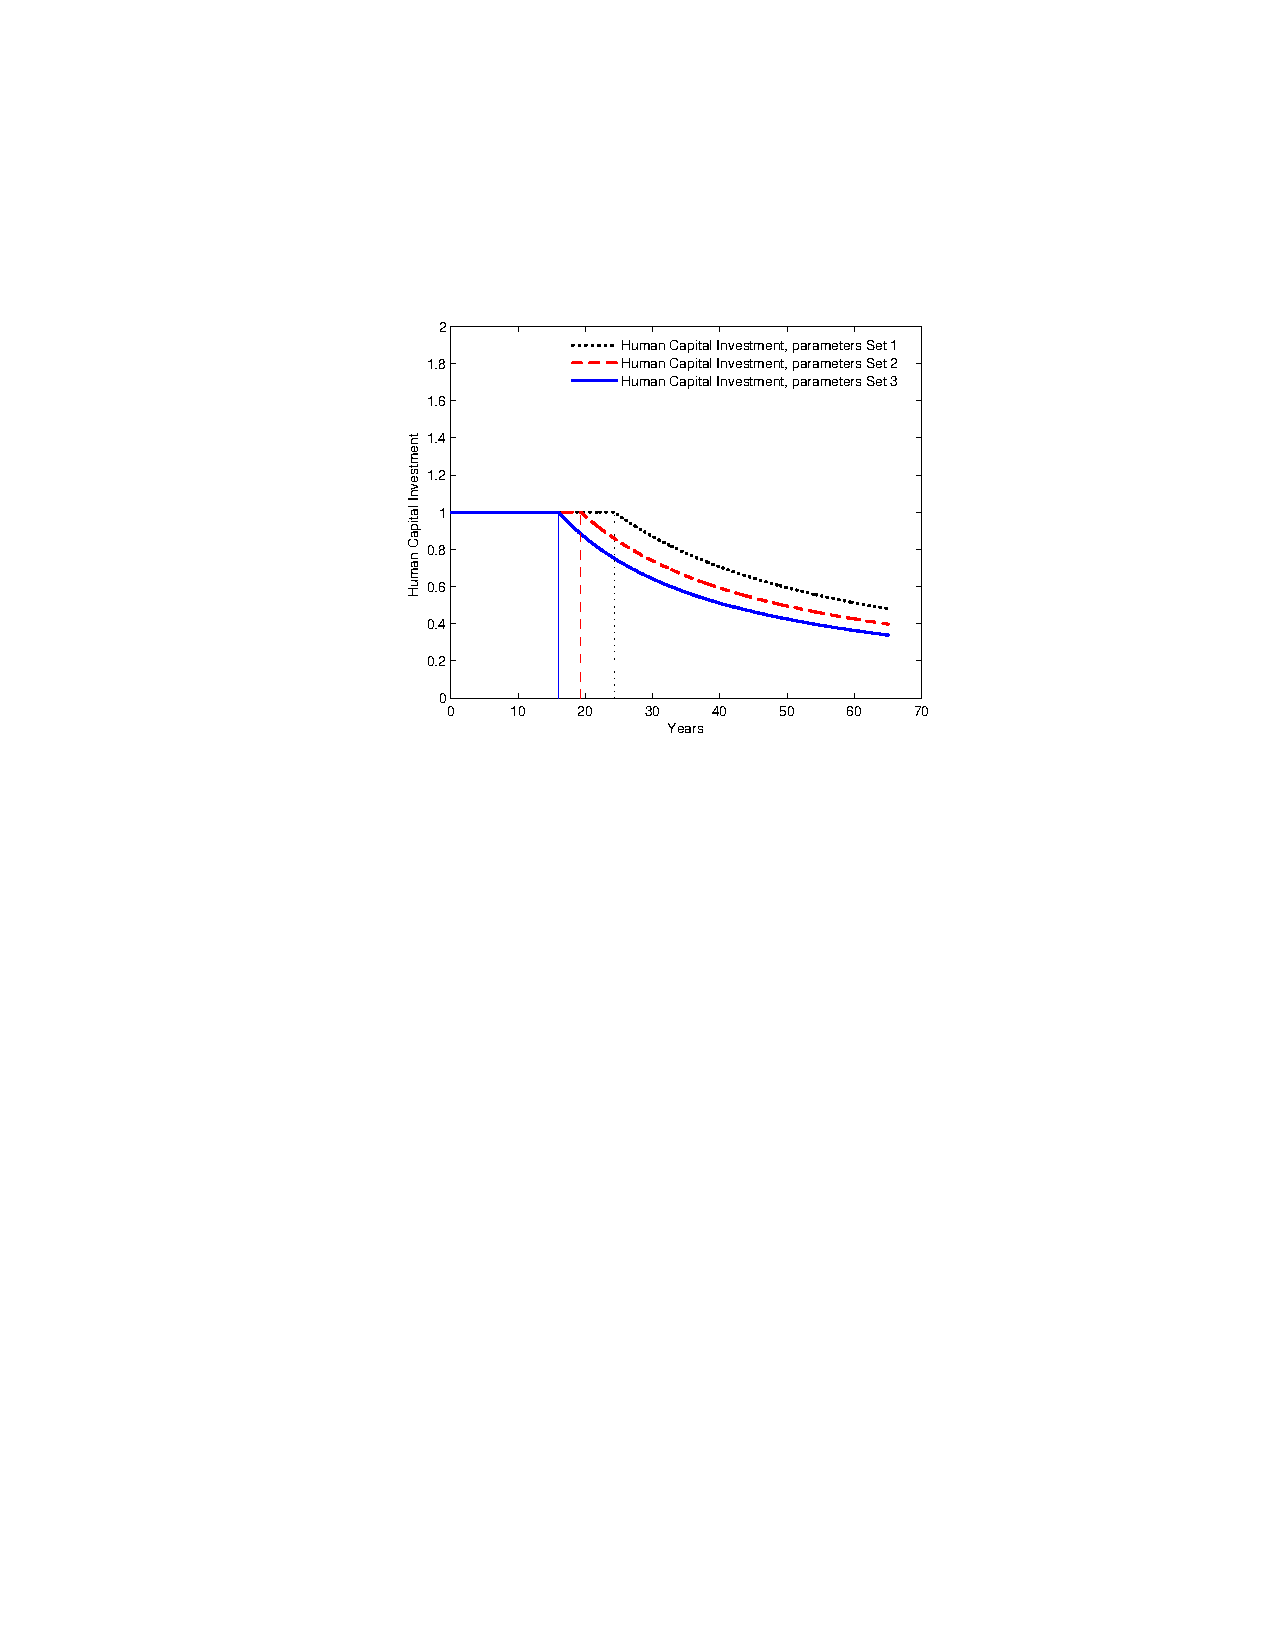
\includegraphics[width=2.2in, height=2.2in]{Figures/fig-hc-earn-series-05.pdf}
        }\\
        \subfigure[Human Capital Stock]{
            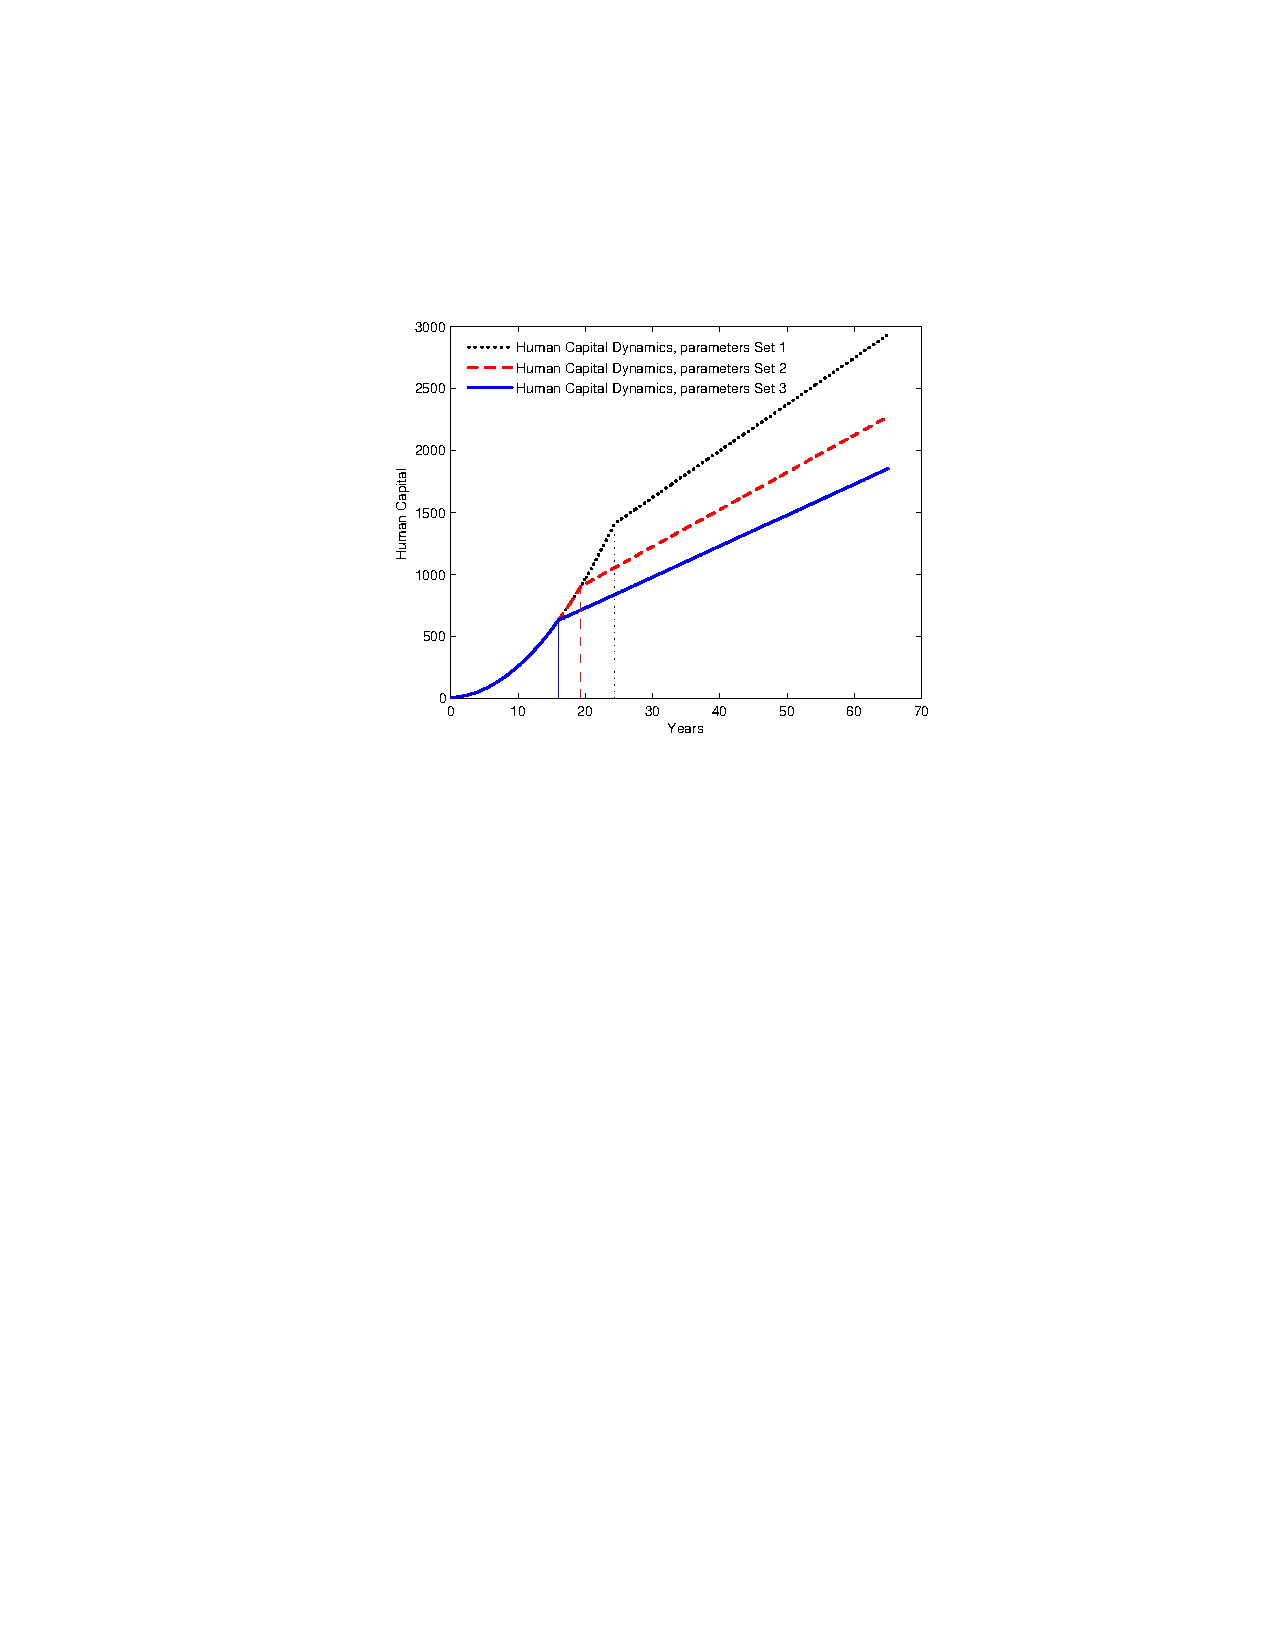
\includegraphics[width=2.2in, height=2.2in]{Figures/fig-hc-earn-series-04.pdf}
        }\\
        \subfigure[Earnings]{%
            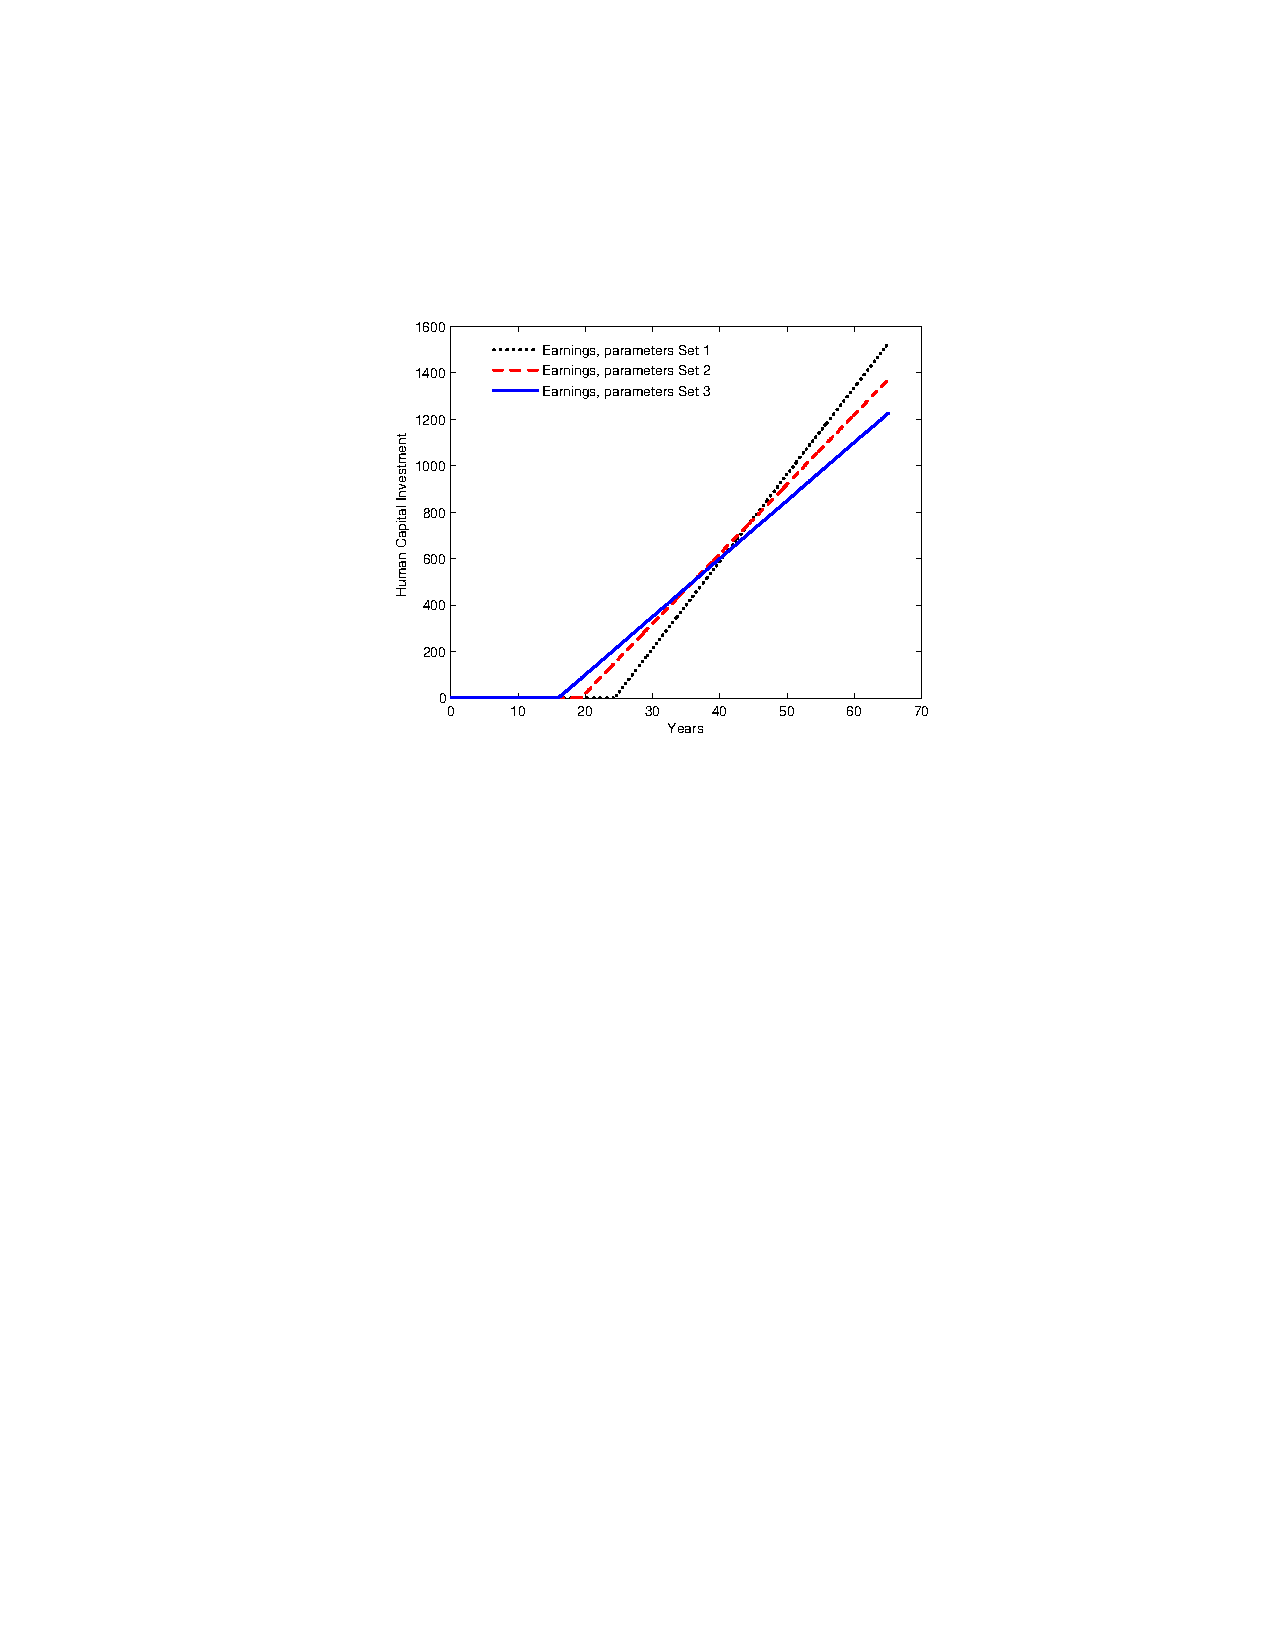
\includegraphics[width=2.2in, height=2.2in]{Figures/fig-hc-earn-series-06.pdf}
        }
    \end{center}
\end{figure}

\begin{figure}[H]
     \begin{center}
   			\caption{Dynamics for $r = .03, \alpha = .5, H_{0} = 10$ \\ $A = .5$ (dotted); $A = 1.0$ (dashed); $A = 1.5$ (solid) }
        \subfigure[Human Capital Investment]{
            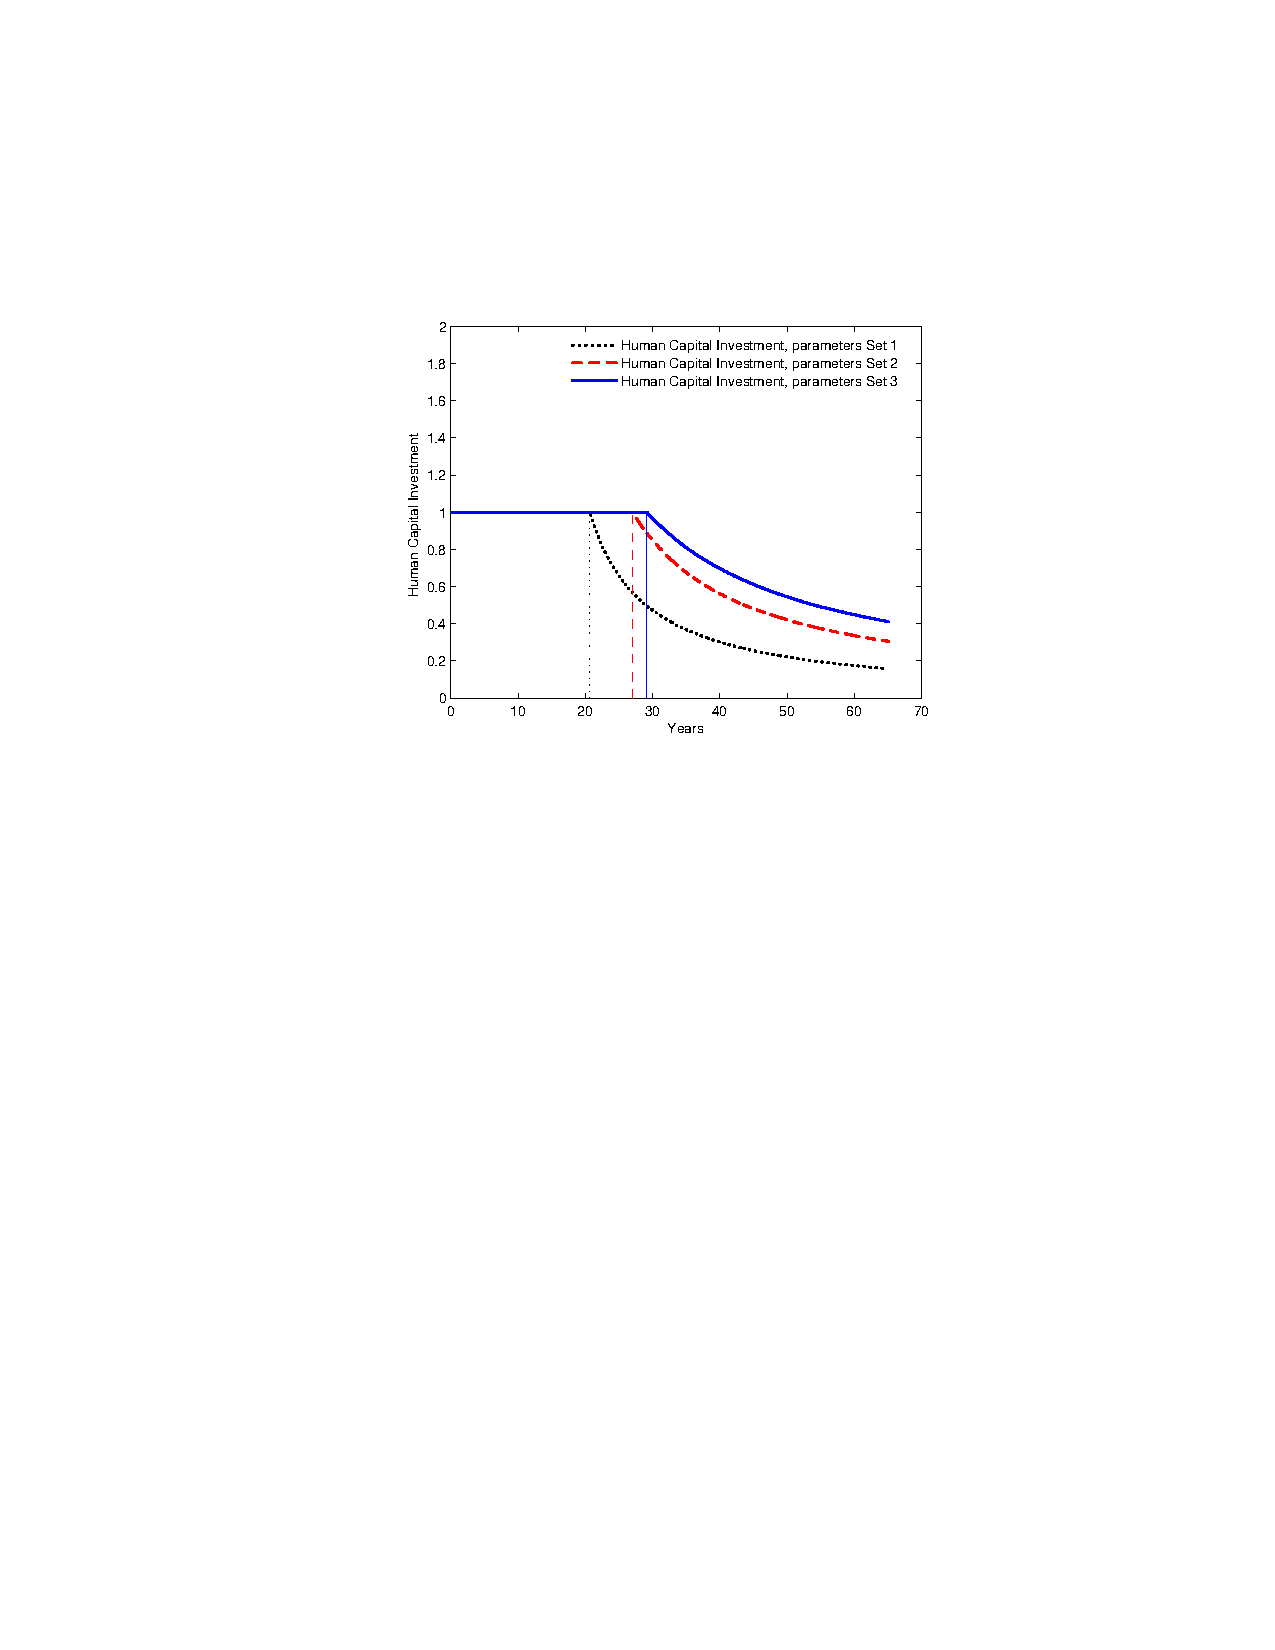
\includegraphics[width=2.2in, height=2.2in]{Figures/fig-hc-earn-series-08.pdf}
        }\\
        \subfigure[Human Capital Stock]{
            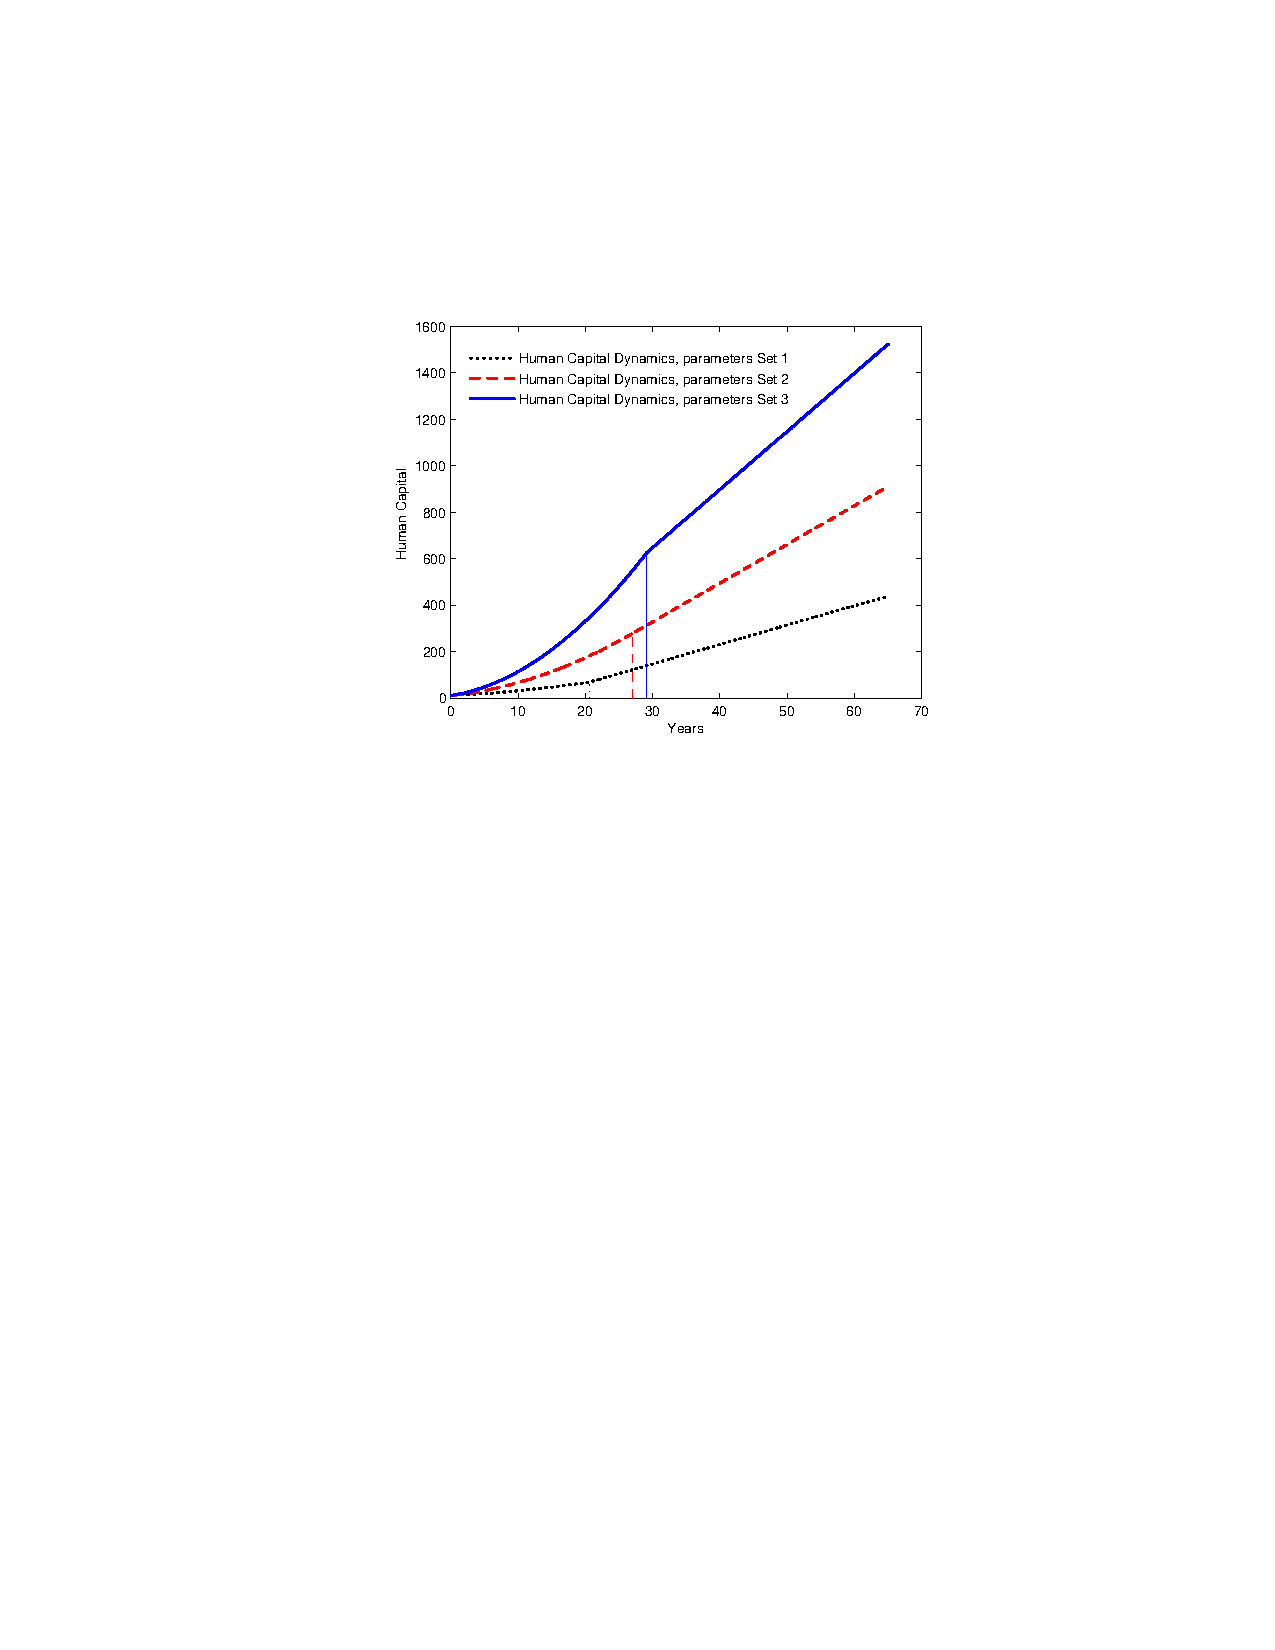
\includegraphics[width=2.2in, height=2.2in]{Figures/fig-hc-earn-series-07.pdf}
        }\\
        \subfigure[Earnings]{%
            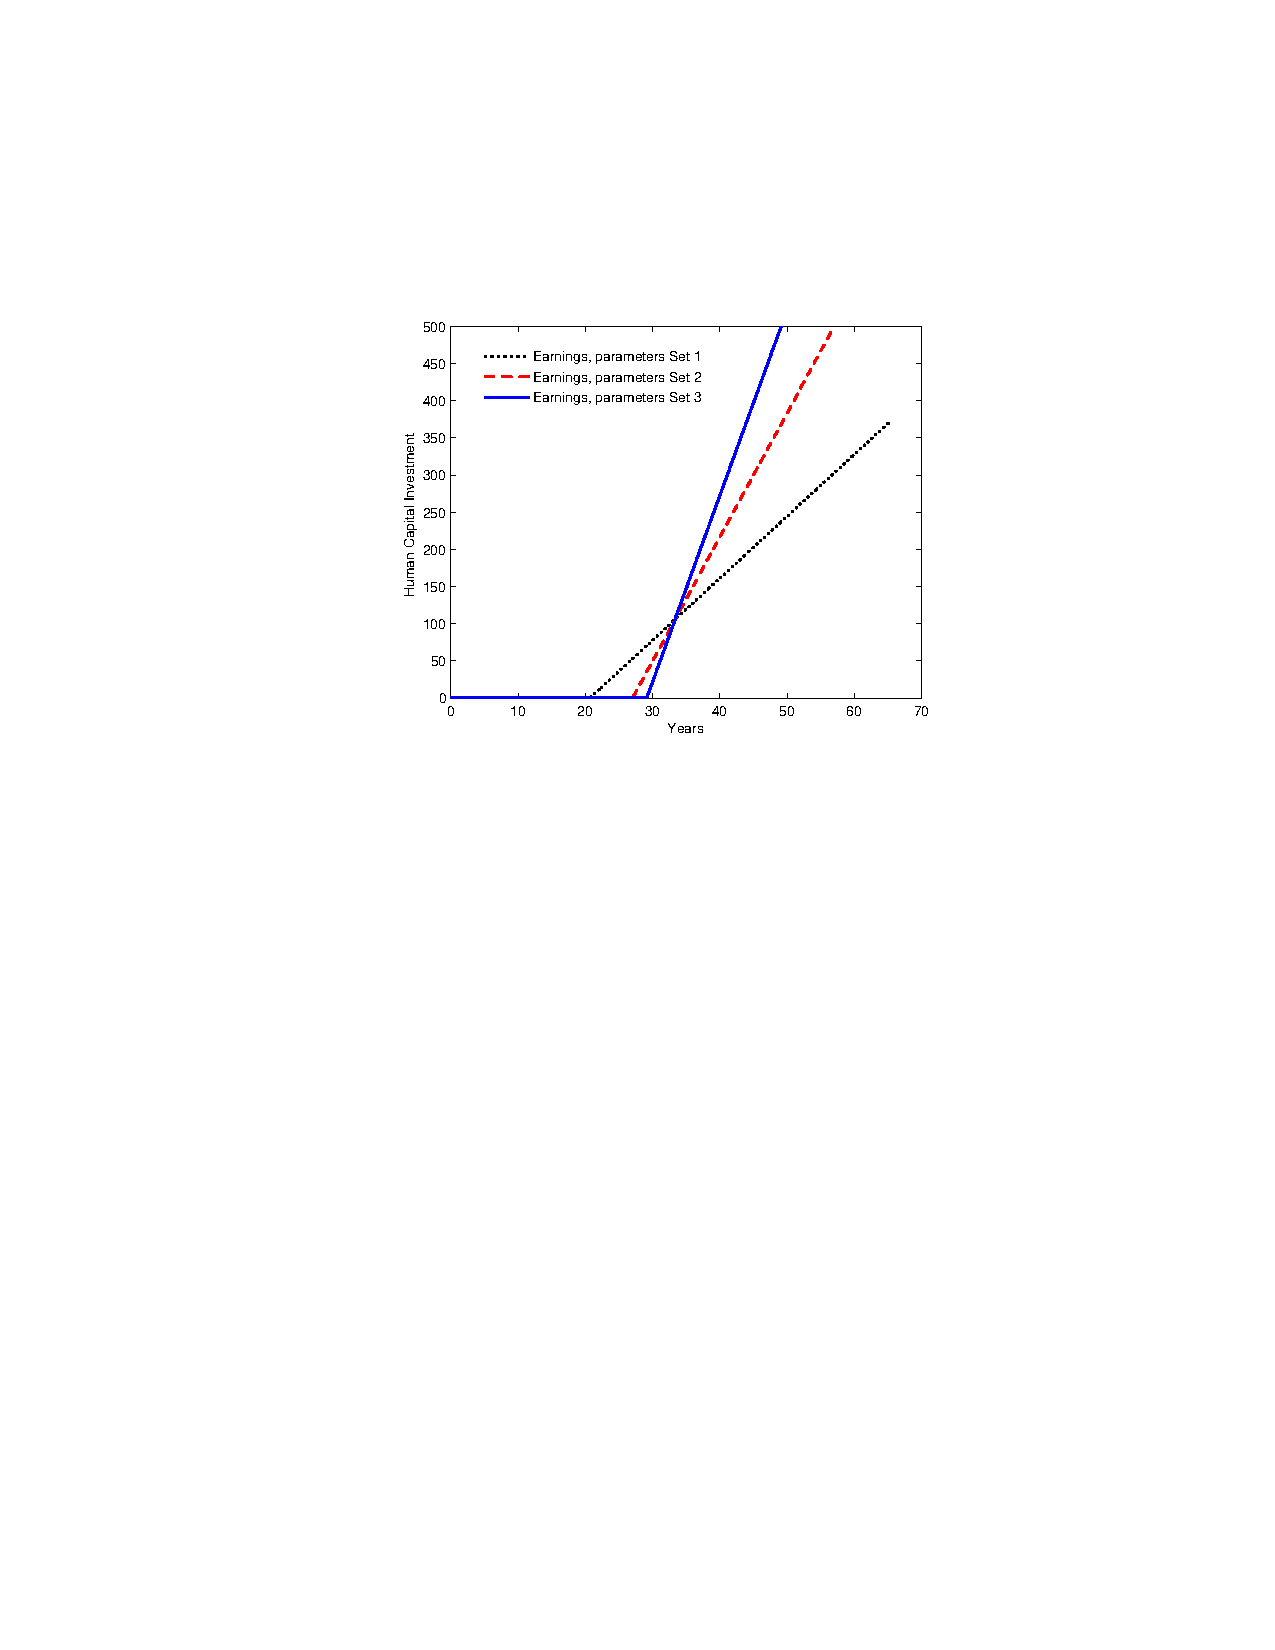
\includegraphics[width=2.2in, height=2.2in]{Figures/fig-hc-earn-series-09.pdf}
        }
    \end{center}
\end{figure}

\begin{figure}[H]
     \begin{center}
    			\caption{Dynamics for $r = .025, \alpha = .5, A = .6$ \\ $H_{0} = 10$ (dotted); $H_{0} = 20$ (dashed); $H_{0} = 30$ (solid)}
        \subfigure[Human Capital Investment]{
            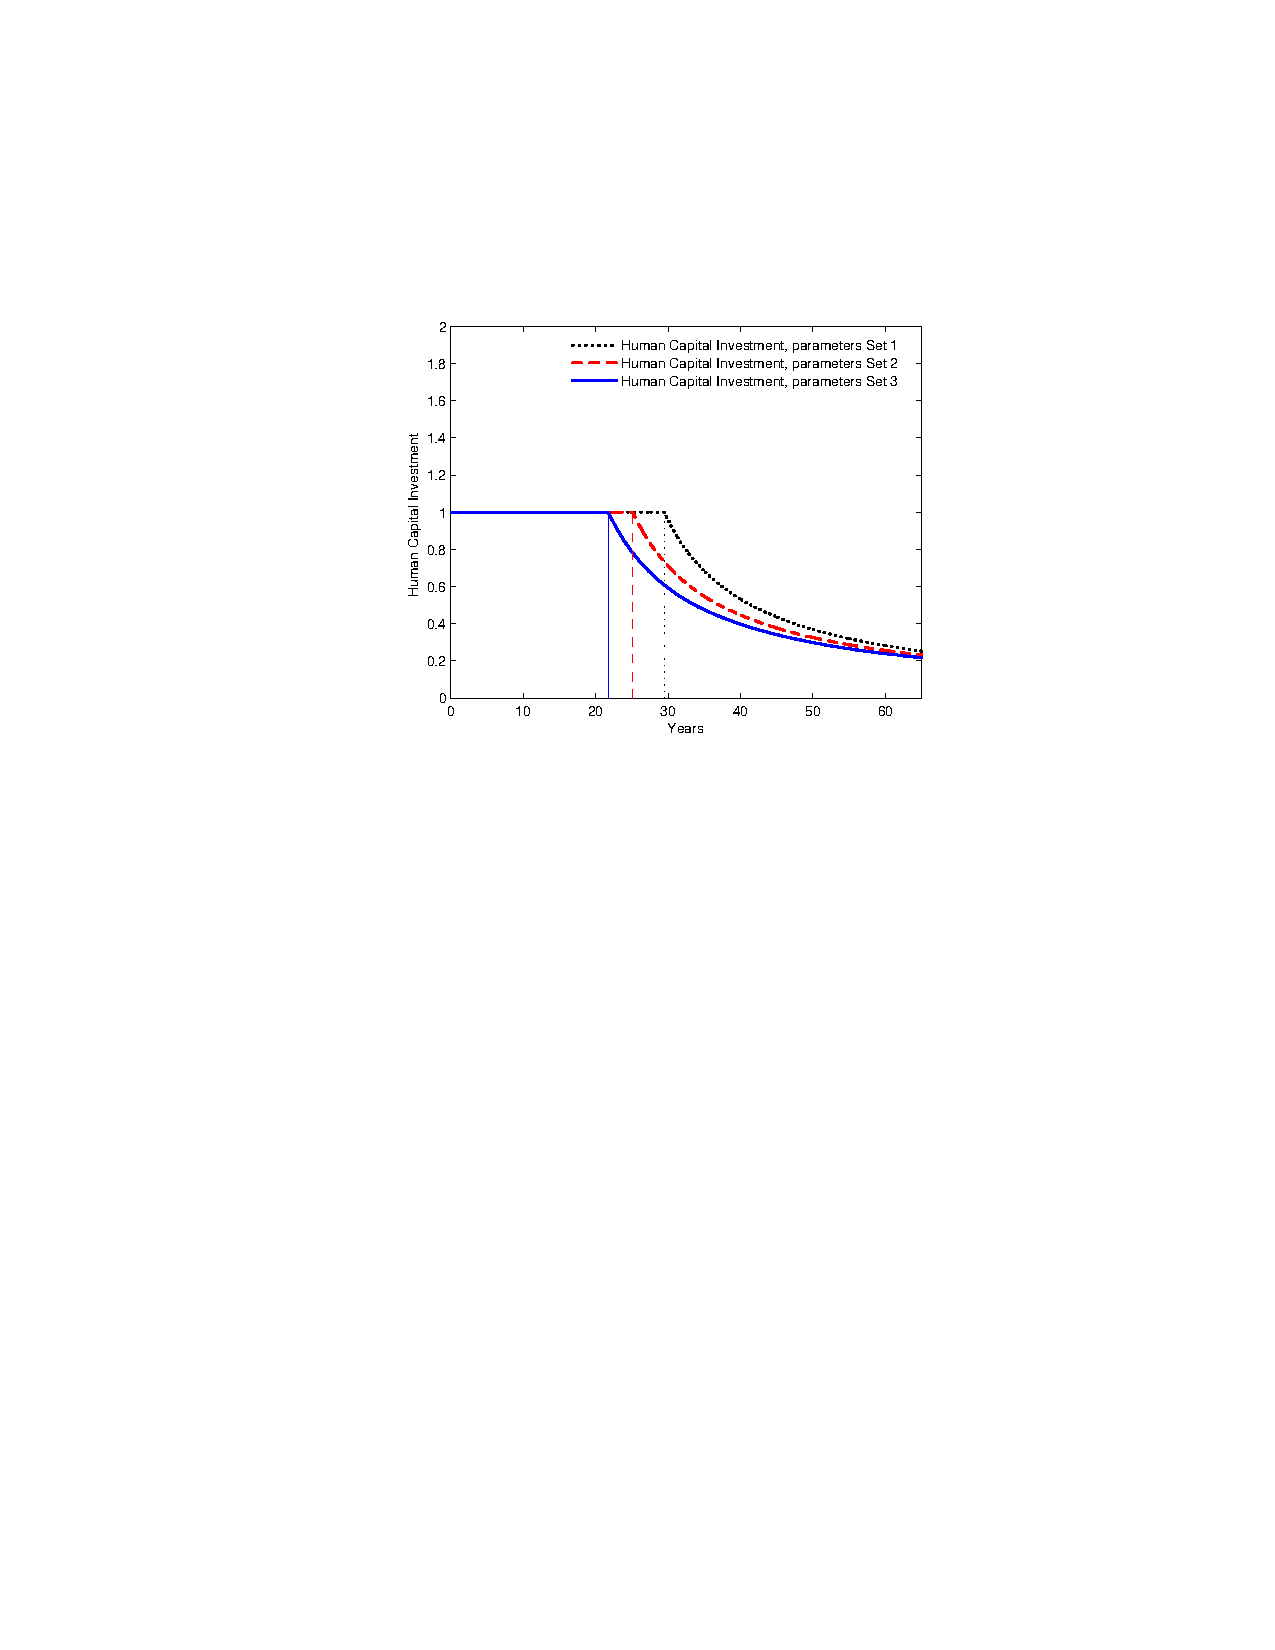
\includegraphics[width=2in, height=2in]{Figures/fig-hc-earn-series-11.pdf}
        }\\
        \subfigure[Human Capital Stock]{
            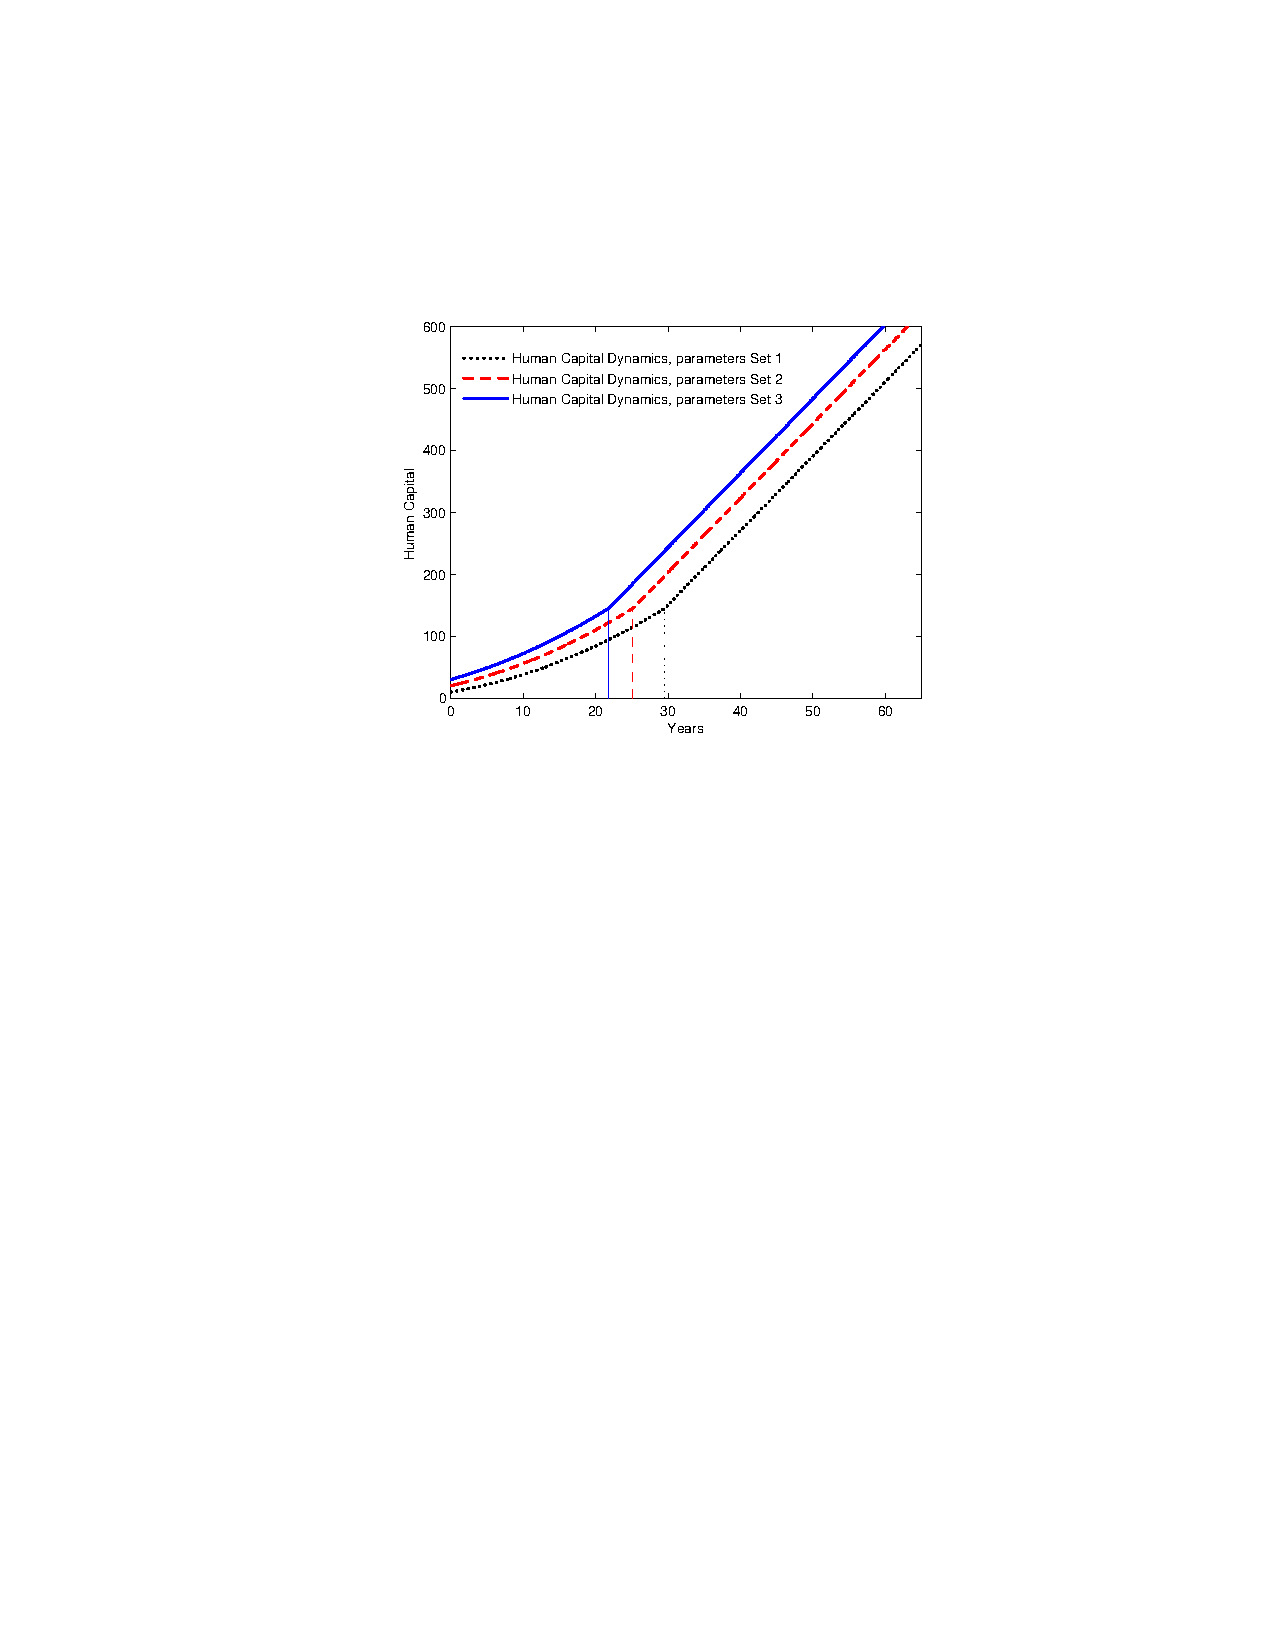
\includegraphics[width=2in, height=2in]{Figures/fig-hc-earn-series-10.pdf}
        }\\
        \subfigure[Earnings]{%
            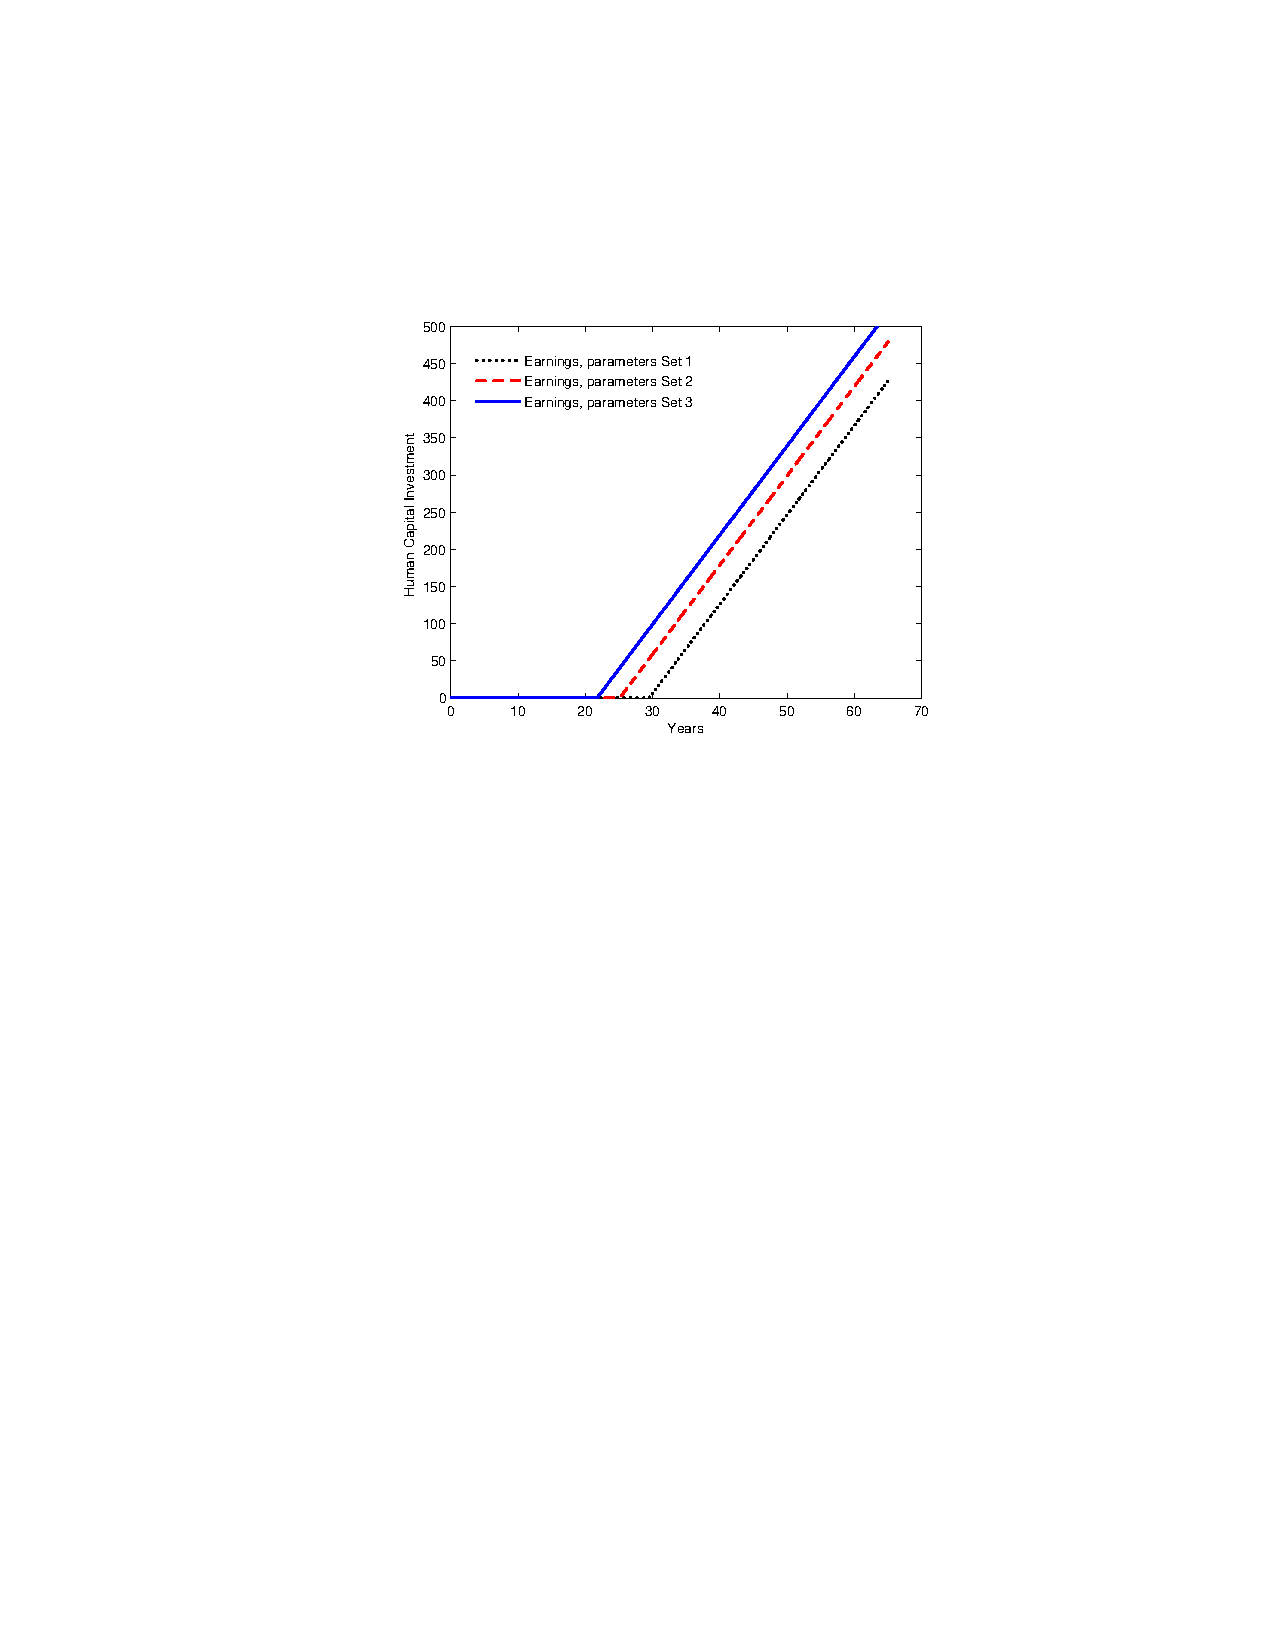
\includegraphics[width=2in, height=2in]{Figures/fig-hc-earn-series-12.pdf}
        }
    \end{center}
\end{figure}

\section{The Haley-Rosen Specification: Finite Horizon and the Autoregression Form}
We analyze the finite horizon case under an specification that \citet{haley1976estimation} and \citet{rosen1976theory} use. Specifically, we assume that $\dot{H} = A \left( IH \right)^{\alpha}, \alpha = \frac{1}{2}, \sigma = 0$ and the exact same setting as in Section \ref{section:baseline}. Actually, in Section \ref{section:baseline} we rely on infinite horizon to derive a set of closed form solutions to the individual's problem. In this section we rely on the assumption $\alpha = \frac{1}{1}$ to do exactly the same.\\
\indent We focus on the dynamics of post-schooling earnings because one of the less credible consequence of the infinite horizon is the linearity of earnings on experience. From \eqref{equation:postearnings} we can write\footnote{Typo there is Appendix slife 89. Confusin $t$ and $\tau$}
\begin{eqnarray}
E(\tau) &=& RH(t^*) + R \int \limits _{0} ^{\tau} A \left[\frac{1}{2} \frac{g(t^* + l)A}{R} \right]dl - R \left[\frac{1}{2} \frac{g(t^* + l)A}{R} \right]^{2} \nonumber \\
&\Rightarrow& \nonumber \\
\dot{E(\tau)} &=& \frac{g (t^* + \tau)A^2}{2R}\left( 2R -rg (t^* + \tau) \right) \nonumber \\
&\Rightarrow& \nonumber \\
\ddot{E(\tau)} &=& -\frac{A^2}{R}\dot{g(t^* + \tau)}^2 \label{eq:earnalpha2}
\end{eqnarray}
where the second and third equalities use \eqref{eq:grossdep}. Combining \eqref{eq:grossdep} and \eqref{eq:earnalpha2} we obtain a second order ODE with constant coefficients:
\begin{equation}
\ddot{E(\tau)} = 2r \dot{E(\tau)} - A^2 R \label{eq:earndifferential}
\end{equation} 

\noindent where the natural initial and terminal conditions that we impose are $E(0)$ and $\ddot{E(T)} = 0$ and then we guess and verify that $c_{2} = \frac{A^2 R}{2r}\exp^{2rT}$ in the following general solution to \eqref{eq:earndifferential}\footnote{There is a typo here in the general solution to the differential equation (slide 50) and in the initial conditions as well. Also, one wrong initial condition is provided.}
\begin{equation}
E(\tau) = c_{0} + c_{1}\exp^{-2r \tau} + c_{2} \tau
\end{equation}

\noindent so that $c_{1} + c_{0} = 0, 2rc_1 \exp^{2rT}  + c_{2} = 0$ and, therefore,
\begin{equation}
E(\tau) = \frac{A^2 R}{4r^2} \exp^{-2r T} \left( 1 - \exp^{2r \tau} \right) + \frac{A^2 R}{2r} \tau. \label{eq:earningspostalpha12}
\end{equation}

\begin{center}
\begin{figure}[H]
\caption{Post-school Earnings in the Haley-Rosen Specification}
\centering
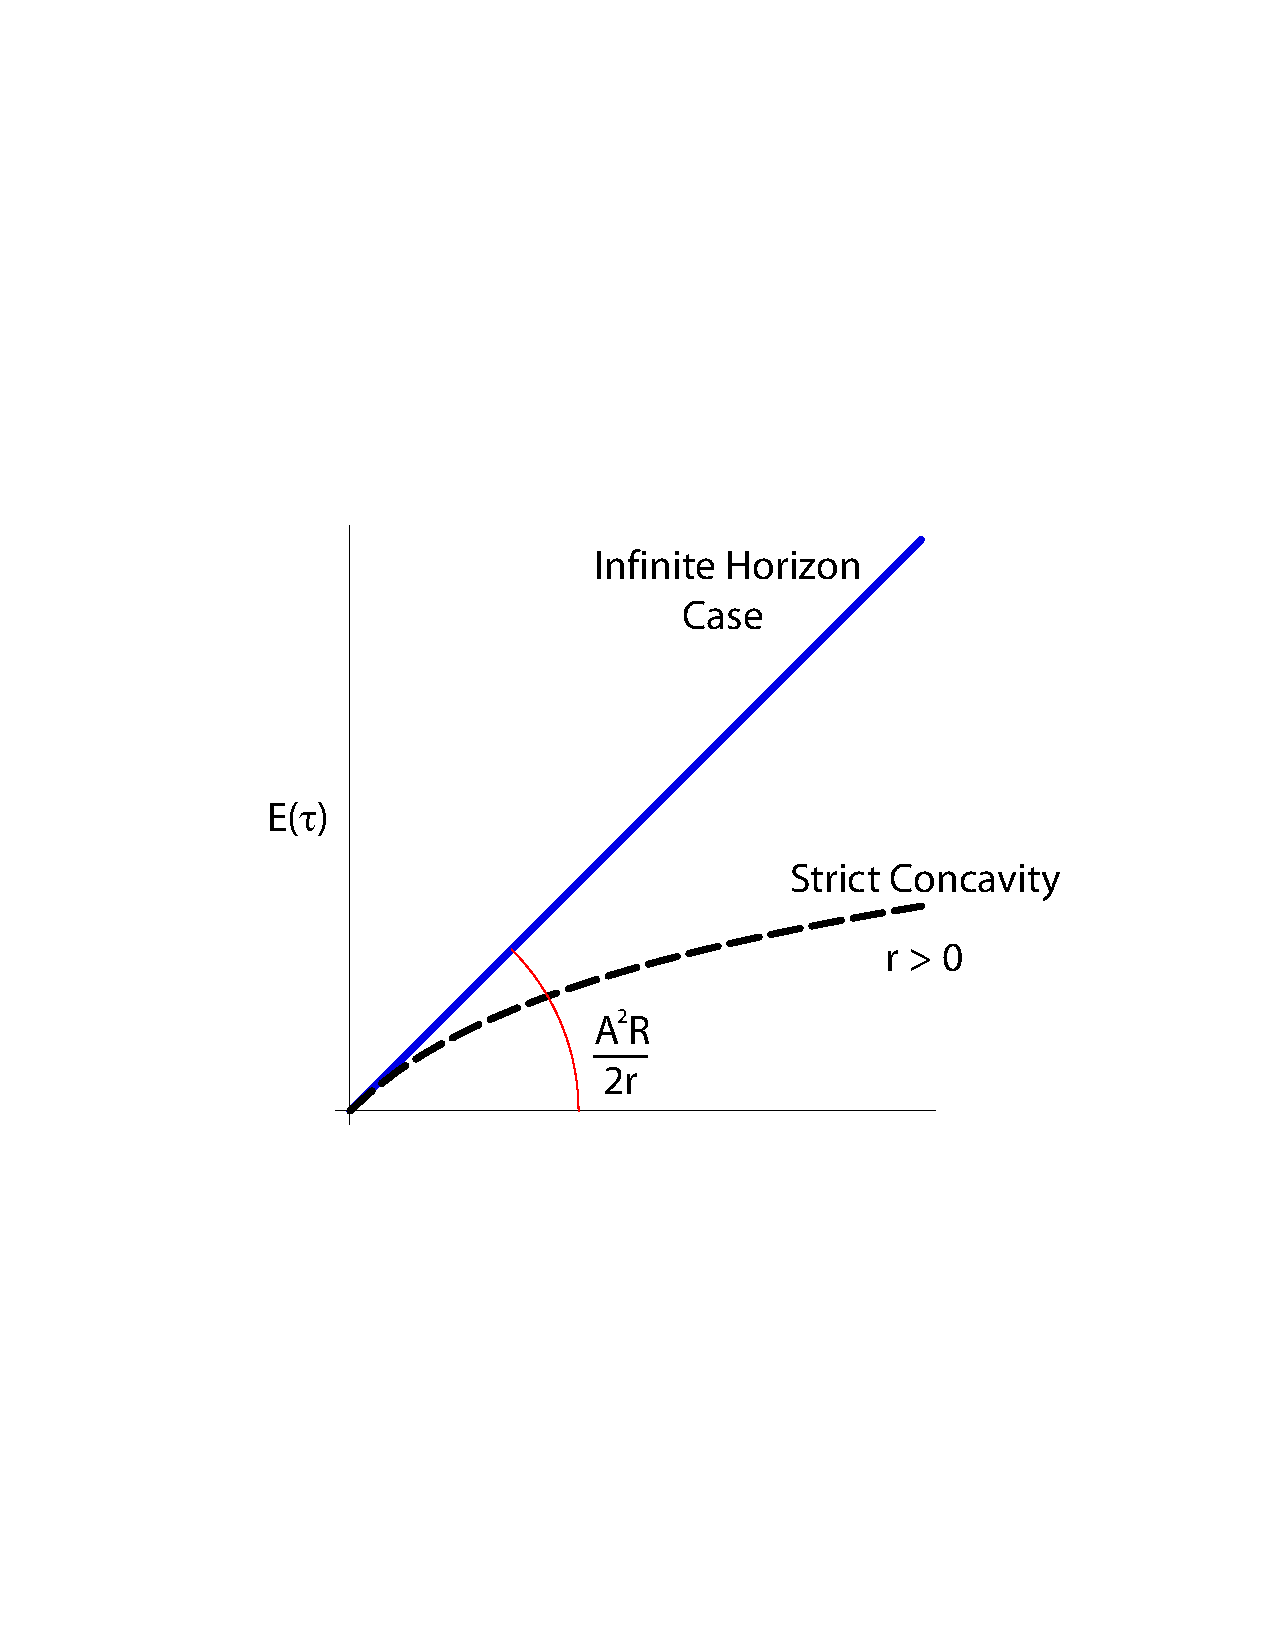
\includegraphics[width=3.5in, height=1.5in]{Figures/fig-finite-horiz.pdf}
\floatfoot{\begin{small}
Note:
\end{small}}
\end{figure}
\end{center}

\indent \textbf{Need to include a discussion here on why this is constant in infinite horizon or $r = 0$.}

\subsection{Evidence}
\citet{brown1976model} estimates \eqref{eq:earningspostalpha12}, which enables to identify $r$ and $A^2 R$. His estimates, however, are imprecise and show that $r \rightarrow 0$. Then, he estimates the model for the infinite horizon case. He claims this to be a good approximation because he has a sample of young individuals. However, this disables him to estimate $r$.

\subsection{The Autoregression}
From \eqref{eq:earningspostalpha12} it is possible to write
\begin{equation}
E(\tau + 1) - E(\tau) =  \frac{A^2 R}{2r}+ \frac{A^2 R}{4r^2} e^{-2rT} \left( \exp^{2r(\tau - 1)} \exp^{r \tau} \right) 
\end{equation}

\noindent which implies that\footnote{slide 55 typo when multiplying by $e^2r$}

\begin{equation}
z(\tau + 1) = e^{2r} z(\tau) + \frac{A^2 R}{2r} \left( 1 - \exp^{2r} \right) \label{eq:growthalpha12}
\end{equation}

\noindent and we can analyze the growth dynamics of earnings. Consider a visual representation of \eqref{eq:growthalpha12}

\begin{center}
\begin{figure}[H]
\caption{Earnings Growth in the Haley-Rosen Representation}
\centering
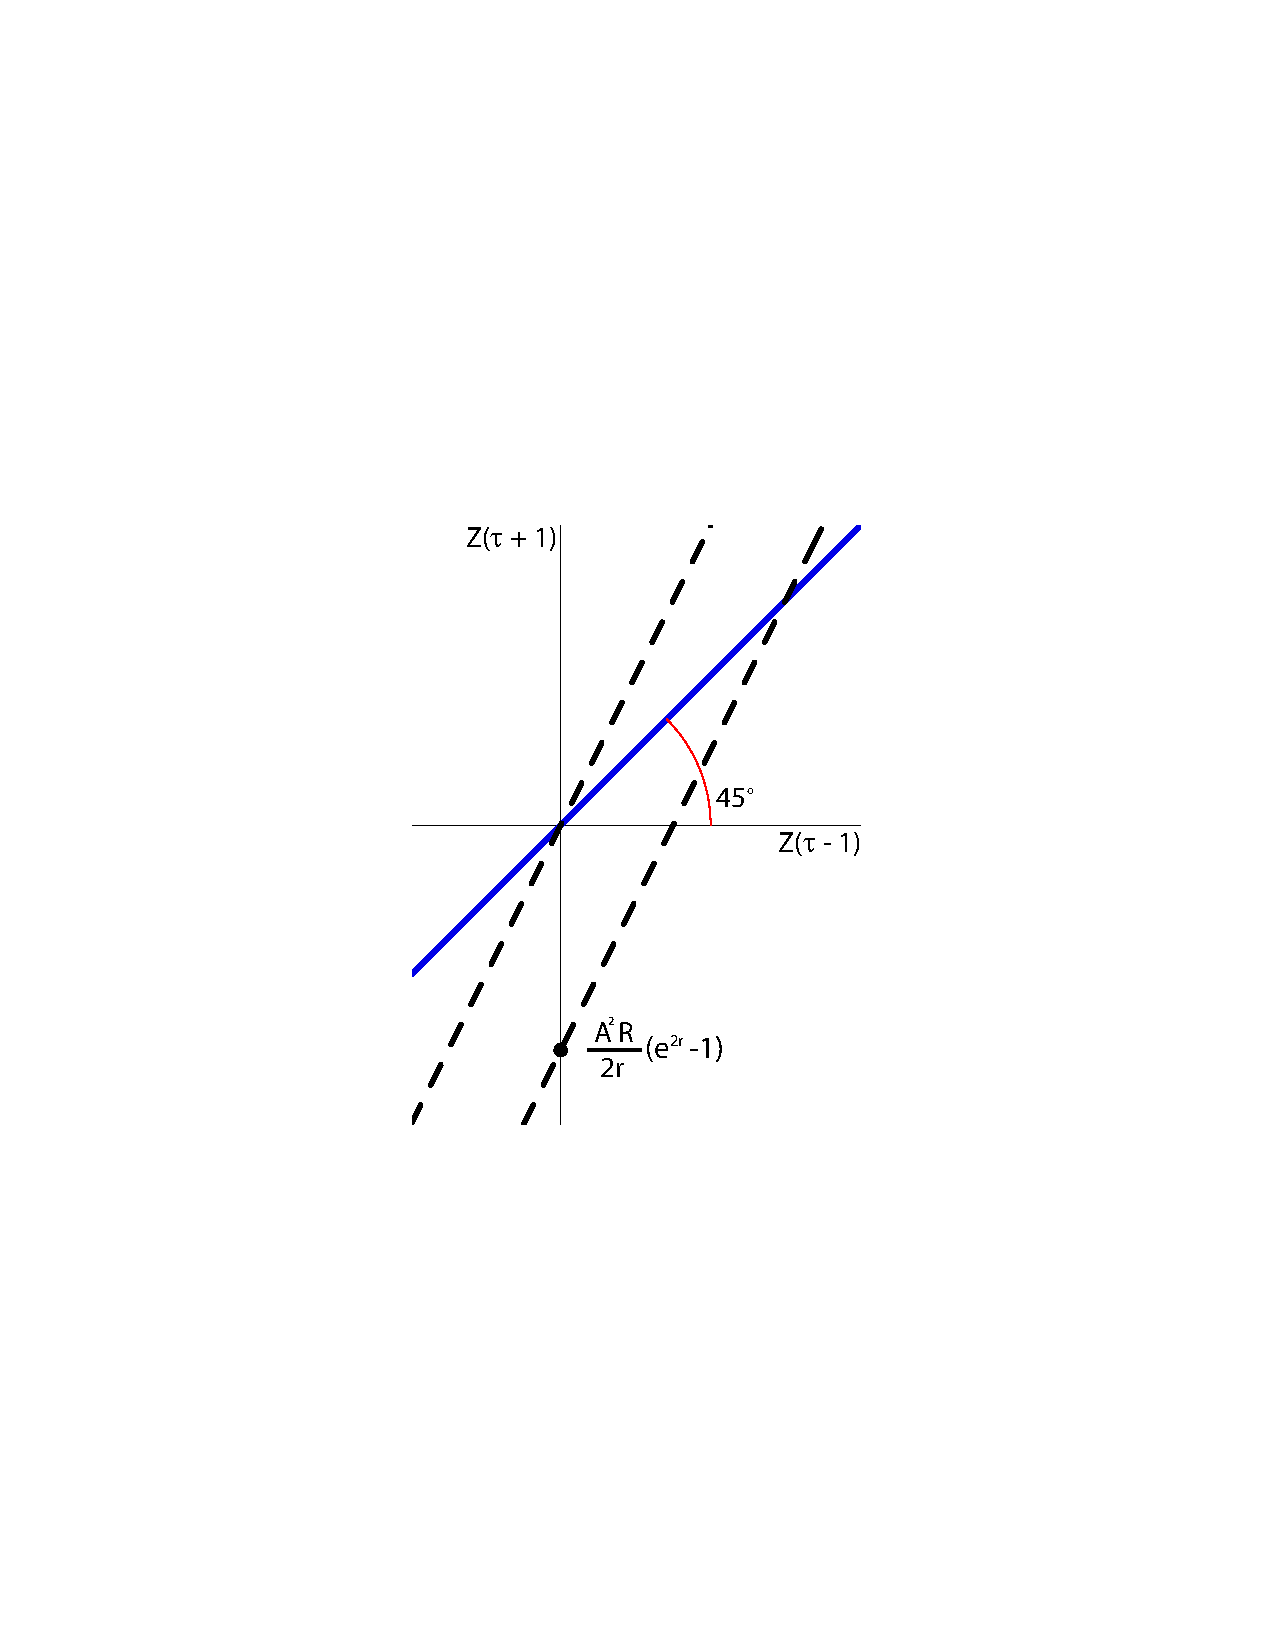
\includegraphics[width=3in, height=3in]{Figures/fig-explode-converge.pdf}
\floatfoot{\begin{small}
Note:
\end{small}}
\end{figure}
\end{center}

\indent Apparently, the dynamics of the earnings growth are explosive. However, note that
\begin{eqnarray}
\frac{\partial \left[ E(\tau) - E(\tau - 1) \right] }{\partial \tau} &=& \frac{A^2 R}{2r} e^{2r(\tau - T)} \left[ \exp^{-2r} - 1 \right] \nonumber \\
&<& 0
\end{eqnarray}
so that even when the growth dynamics of earnings is autoregressive it converges to a constant. More formally, note that $z(0) = E(0) \equiv z_{0}$ and solve \eqref{eq:growthalpha12} to get
\begin{equation}
z(\tau) = \exp^{2rT} z_{0} + \frac{A^2 R}{2r} \left( 1 - e^{2r} \right) \sum \limits _{j=0} ^{T-1} \exp^{2rj}
\end{equation}

\noindent so that the earnings growth converges to the constant $\exp^{2rT} z_{0}$.\\

\subsection{From the Haley-Rosen Specification to the Mince Equation}
The earnings function in the Haley-Rosen specification actually leads to the Mincer equation. To see that take take logs of \eqref{eq:earningspostalpha12} and obtain
\begin{equation}
\ln E(\tau) = \ln \left( \frac{A^2 R}{ 2r} \right) + \ln \tau + \ln \left[ 1 + \frac{\exp^{-2rT} - \exp^{2r(\tau - T)} }{2r \tau} \right]. \label{eq:logs}
\end{equation}

\indent We can approximate around $\tau_{0}$ the second and third terms in \eqref{eq:logs} to obtain
\begin{eqnarray}
\ln(\tau) &\approx& \ln (\tau_{0}) + \frac{1}{\tau_{0}} \left( \tau - \tau_{0} \right) - \frac{1}{\tau_{0}^2} \frac{\left( \tau - \tau_{0} \right)^2}{2!} \nonumber \\
\ln \left[ 1 + \frac{\exp^{-2rT} - \exp^{2r(\tau - T)} }{2r \tau} \right] &\approx& \xi_{0} + \xi_{1} \left( \tau - \tau_{0} \right) + \xi_{2} \frac{\left( \tau - \tau_{0} \right)^2}{2!}
\end{eqnarray}

\noindent for the adequate $\xi_{0}, \xi_{1}, xi_{2}$. Thus,
\begin{equation}
\ln(\tau) + \ln \left[ 1 + \frac{\exp^{-2rT} - \exp^{2r(\tau - T)} }{2r \tau} \right] \approx \alpha_{0} + \alpha_{1}\left( \tau - \tau_{0} \right) + \alpha_{2} \left( \tau - \tau_{0} \right)^2
\end{equation}

\noindent with $\alpha_{0} \equiv = \ln(\tau_{0}) + \xi_{0}, \alpha_{1} \equiv \frac{1}{\tau_{0}} + \xi_{1}, \alpha_{2} \equiv \frac{-\frac{1}{\tau_{0}^2} + \xi_{2}}{2}$. This leads to the so called Mincer equation \citep[see][]{mincer1974schooling}:
\begin{equation}
\ln E(\tau) = k_{0} + k_{1} \tau k_{2} \tau^2 \label{eq:mincer}
\end{equation}

\noindent where $k_{0} = \alpha_{0} - \tau_{0} \alpha_{1} + \alpha_{2} \tau_{0}^2, k_{2} = \alpha_{2}$. This provides a baseline to compare ``Ben-Porath'' with ``Mincer'' coefficients. Table \ref{table:bpmincer} provides different combinations of the parameters $r, \tau_{0}, T$ that lead to different values of $k_{1}, k_{2}$ that are close to the estimates that \citet{mincer1974schooling} obtains.

\begin{center}
\begin{table}[H]
\begin{threeparttable}
\fontsize{9}{12pt}\selectfont
\caption{The Ben-Porath and the Mincer Coefficients} \label{table:bpmincer}
\centering
\begin{tabular}{ccc|cc}
\multicolumn{3}{c|}{Parameters} & \multicolumn{2}{c}{Ben Porath
Coefficients} \\ \hline\hline $r$ & $\tau _{0}$ & $T$ & $k_{1}$ &
$k_{2}$ \\ \hline $0.0225$ & $29.54$ & $41.43$ & $0.081$ & $-0.0010$
\\ \hline $0.05$ & $25$ & $60$ & $0.0808$ & $-0.0008$ \\ \hline
$0.05$ & $20$ & $65$ & $0.1002$ & $-0.0013$ \\ \hline $0.0675$ &
$24.70$ & $74.77$ & $0.081$ & $-0.0008$ \\ \hline\hline
\multicolumn{3}{c}{Mincer Coefficients} & $0.081$ & $-0.0012$ \\
\hline
\end{tabular}
\begin{tablenotes}
\small
\item Note: the Mincer model or Mincer equation is $\ln ( \text{E} ) =k_{0}+k_{1}\tau +k_{2}\tau^{2}$, where $\tau$ is experience.  
\end{tablenotes}
\end{threeparttable}
\end{table}
\end{center}

Now, if $rT \approx 0$ then $\exp^{-rT} \approx 1$ and \eqref{eq:logs} becomes 
\begin{equation}
\ln E(\tau) \approx \ln \left( \frac{A^2 R}{2r} \right) + \ln \tau + \ln \left[ 1 + \frac{1 - \exp^{2r \tau}}{2 r \tau} \right] \label{eq:intercept}
\end{equation}

which leads to various observations. The Haley-Rosen specification of the Ben-Porath model implies no economic content for the Mincerian rate of return on post-school investment. Put differently, an extension of \eqref{eq:mincer} which includes post-school investment does not have a structural counterpart. Actually, this model implies that the entire economic content is in the intercept (see \eqref{eq:intercept}. Actually, \eqref{eq:intercept} implies that, \textit{caeteris paribus}, schooling has no effect on earnings. \citet{mincer1974schooling} finds that the contrary. However, we claim that his finding does not necessarily argues against the Ben-Porath model. It could simply be the case that \citet{mincer1974schooling} does not include ability measures in his estimations, which appear in \eqref{eq:intercept}, and therefore finds a positive coefficient on schooling. 

\section{Rates of Return}
We analyze the rate of return to schooling and post-schooling investments based on the model in Section \ref{section:baseline}. Recall that this model considers no depreciation, $\sigma = 0$, and $T \rightarrow \infty$.\footnote{Recall that this implies that $g(t) = \frac{R}{r}$}.
\subsection{Post-school Investment}
Let $E(\tau)^{NPS}$ and $E(\tau)^{PS}$ denote earnings without and with post-schooling investment, respectively. By \eqref{eq:earnsall} we can write
\begin{eqnarray}
E(\tau)^{NPS} &=& R H(t*) \\ \nonumber
&=& R \left( \frac{\alpha A}{r} \right)^{\frac{1}{1 - \alpha}} \\ \nonumber
E(\tau)^{PS} &=& \left[ \frac{\alpha A}{r} \right]^{\frac{\alpha}{1-\alpha}} \tau
\end{eqnarray}

\noindent so that the increment in earnings due to post-schooling at $\tau$ is

\begin{eqnarray}
\Delta^{E(\tau)} \equiv E(\tau)^{PS} - E(\tau)^{NPS}.
\end{eqnarray}

\indent Actually, is we note that $E(\tau)^{PS} = IH(\tau)$ (see \eqref{eq:itcobb}) then we can interpret $\Delta^{E(\tau)}$ as ``returns less costs'' from post-schooling and let $\phi$ be the (internal) rate of return to post-schooling which solves for
\begin{equation}
\int \limits _{0} ^{\infty} \exp^{- \phi \tau} \left[ \left[ \frac{\alpha A}{r} \right]^{\frac{\alpha}{1-\alpha}} \tau - R \left( \frac{\alpha A}{r} \right)^{\frac{1}{1 - \alpha}} \right] d \tau = 0 \label{eq:postreturn}
\end{equation}  

\noindent Using the Laplace transform, \eqref{eq:postreturn} implies
\begin{eqnarray}
\frac{1}{\phi^2} RA \left[ \frac{\alpha A}{r} \right]^{\frac{\alpha}{1-\alpha}} + \frac{1}{\phi} A \left[ \frac{\alpha A}{r} \right]^{\frac{1}{1-\alpha}} &=& 0 \nonumber \\
&\Rightarrow& \nonumber \\
\phi &=& \frac{r}{\alpha}
\end{eqnarray}

\indent The (internal) rate of return to post-schooling investment is a decreasing function of $\alpha$. Individuals who are more productive require a smaller return in order to invest in the post-school period. Likewise, relatively patient individuals (relatively low $r$) require a smaller $\phi$ to invest in the post-schooling period. 

\subsection{School Investment}
Each $\tau$, an individual with no schooling earns $R H_{0}$ while he earns $R \left[ \frac{\alpha A}{r} \right]^{\frac{1}{1-\alpha}}$ with schooling and no post-schooling. Let $\varphi$ be the (internal) rate of return to schooling be defined as the value $\varphi$ that solves for\footnote{Typo in slide 74 in the definition of what do schooling people earn.}
\begin{eqnarray}
\int _{t^*} ^{\infty} \exp^{- \varphi t} R \left[ \frac{\alpha A}{r} \right]^{\frac{1}{1-\alpha}} dt &=& \int \limits _{0} ^{\infty} \exp^{- \varphi t} R H_{0} dt \nonumber \\
&\Rightarrow& \nonumber \\
\varphi &=& \frac{\ln \left[ \frac{\alpha A}{r} \right]^{\frac{1}{1 - \alpha}} - \ln H_{0}}{\frac{1}{r} - \frac{1}{2} \frac{H_{0}^{\frac{1}{2}}}{A}}
\end{eqnarray}
 
\section{Earnings Growth and Patience in Finite Horizon}
In Section \ref{section:baseline} that relative patience (i.e., relatively low $r$) implies a relatively longer schooling period, relatively higher human capital accumulation, and a relatively steeper earnings profile. We now want to ask, in the same framework but with finite horizon, how earnings growth depends on relative patience. In order to answer that we investigate the behavior of $\frac{\partial \dot{E(\tau)}}{\partial r}$. Without loss of generality, assume that R =1 and note that\\
\indent Note that
\begin{equation}
\frac{\partial \dot{E(\tau)} }{\partial r} = F'(\cdot) \frac{\partial IH}{\partial r} - \frac{\partial}{\partial r} \dot{IH}. \label{eq:earnpartialr}
\end{equation}

\noindent From \eqref{eq:newfocs} we know that the first order condition of the agent's problem is
\begin{equation}
g(t) F'(\cdot) = 1.
\end{equation}

\noindent which by the implicit function theorem yields
\begin{eqnarray}
\frac{\partial IH}{\partial r} &=& \frac{\frac{\partial g(t)}{\partial r} F'(\cdot)}{2 g(t) F''(\cdot)} \nonumber \\ 
&<& 0
\end{eqnarray}

\noindent where the inequality follows from strict concavity of $F(\cdot)$ and  $\ g(t) > 0, \frac{\partial g(t)}{ \partial r} <0$ (see \eqref{eq:partialgr}). Thus, the first term in \eqref{eq:earnpartialr} is negative. If we show that the second term is negative then we can sign \eqref{eq:earnpartialr} and provide a meaning for this results. In order to do that we need $\frac{\partial \dot{IH}}{\partial r} > 0$. From \eqref{eq:itdot} note that 
\begin{equation}
\frac{\partial \dot{IH}}{\partial r} = -\frac{\dot{g}}{g} \left[ 1 - \frac{F'(\cdot)F'''(\cdot)}{{F''(\cdot)}^2}\right] \frac{\partial IH}{\partial r} + \frac{F'(\cdot)}{F''(\cdot)}\frac{\partial}{\partial r} \left[ - \frac{\dot{g}}{g} \right] \label{eq:ihdotr}
\end{equation}

\indent From Section \ref{section:egdyn} we know that a sufficient condition for earnings strict concavity, i.e. $\ddot{E} < 0$ is $1 - \frac{F'(\cdot) F'''(\cdot)}{{F''}^2} < 0$. This together with $\dot{g}, \frac{\partial IH}{\partial r} < 0$ implies that the first term in \eqref{eq:ihdotr} is positive. To sign the second term note that $\dot{g} = rg - 1, - \frac{\dot{g}}{g} = \frac{1}{g} - r$. Then,
\begin{equation}
\frac{\partial}{\partial r} \left[ - \frac{\dot{g}}{g} \right] = - \frac{1}{g^2} \frac{\partial g}{\partial r} - 1. \label{eq:dotgg}
\end{equation}

\indent To sign \eqref{eq:dotgg} note that
\begin{eqnarray}
\frac{\partial g}{\partial r} &=& \frac{\exp^{r(t-T)} \left( 1 - r(t - T) \right) - 1 }{r^2} \nonumber \\
&<& 0 \label{eq:partialgr}
\end{eqnarray}

\noindent and

\begin{eqnarray}
- \frac{\partial g }{g^2 \partial r} - 1 &=& \frac{1}{r^2g^2} \exp^{r(t-T)} \left( 1 + r(t - T) - \exp^{r(t-T)} \right). \nonumber \\
&<& 0
\end{eqnarray}

\indent Therefore, if the earnings function is concave, $\frac{\partial \dot{OH}}{\partial r} > 0$ which implies that $\frac{\partial \dot{E}}{\partial r} < 0$. This implies that the earnings function is relatively ``less concave'' for relatively impatient individuals (relatively high $r$). This is a consequence of their investment decisions: they spent less time in the schooling period and accumulate less human capital.

\begin{center}
\begin{figure}[H]
\caption{Earnings Profiles in Finite Horizon for Different Values of $r$ }
\centering
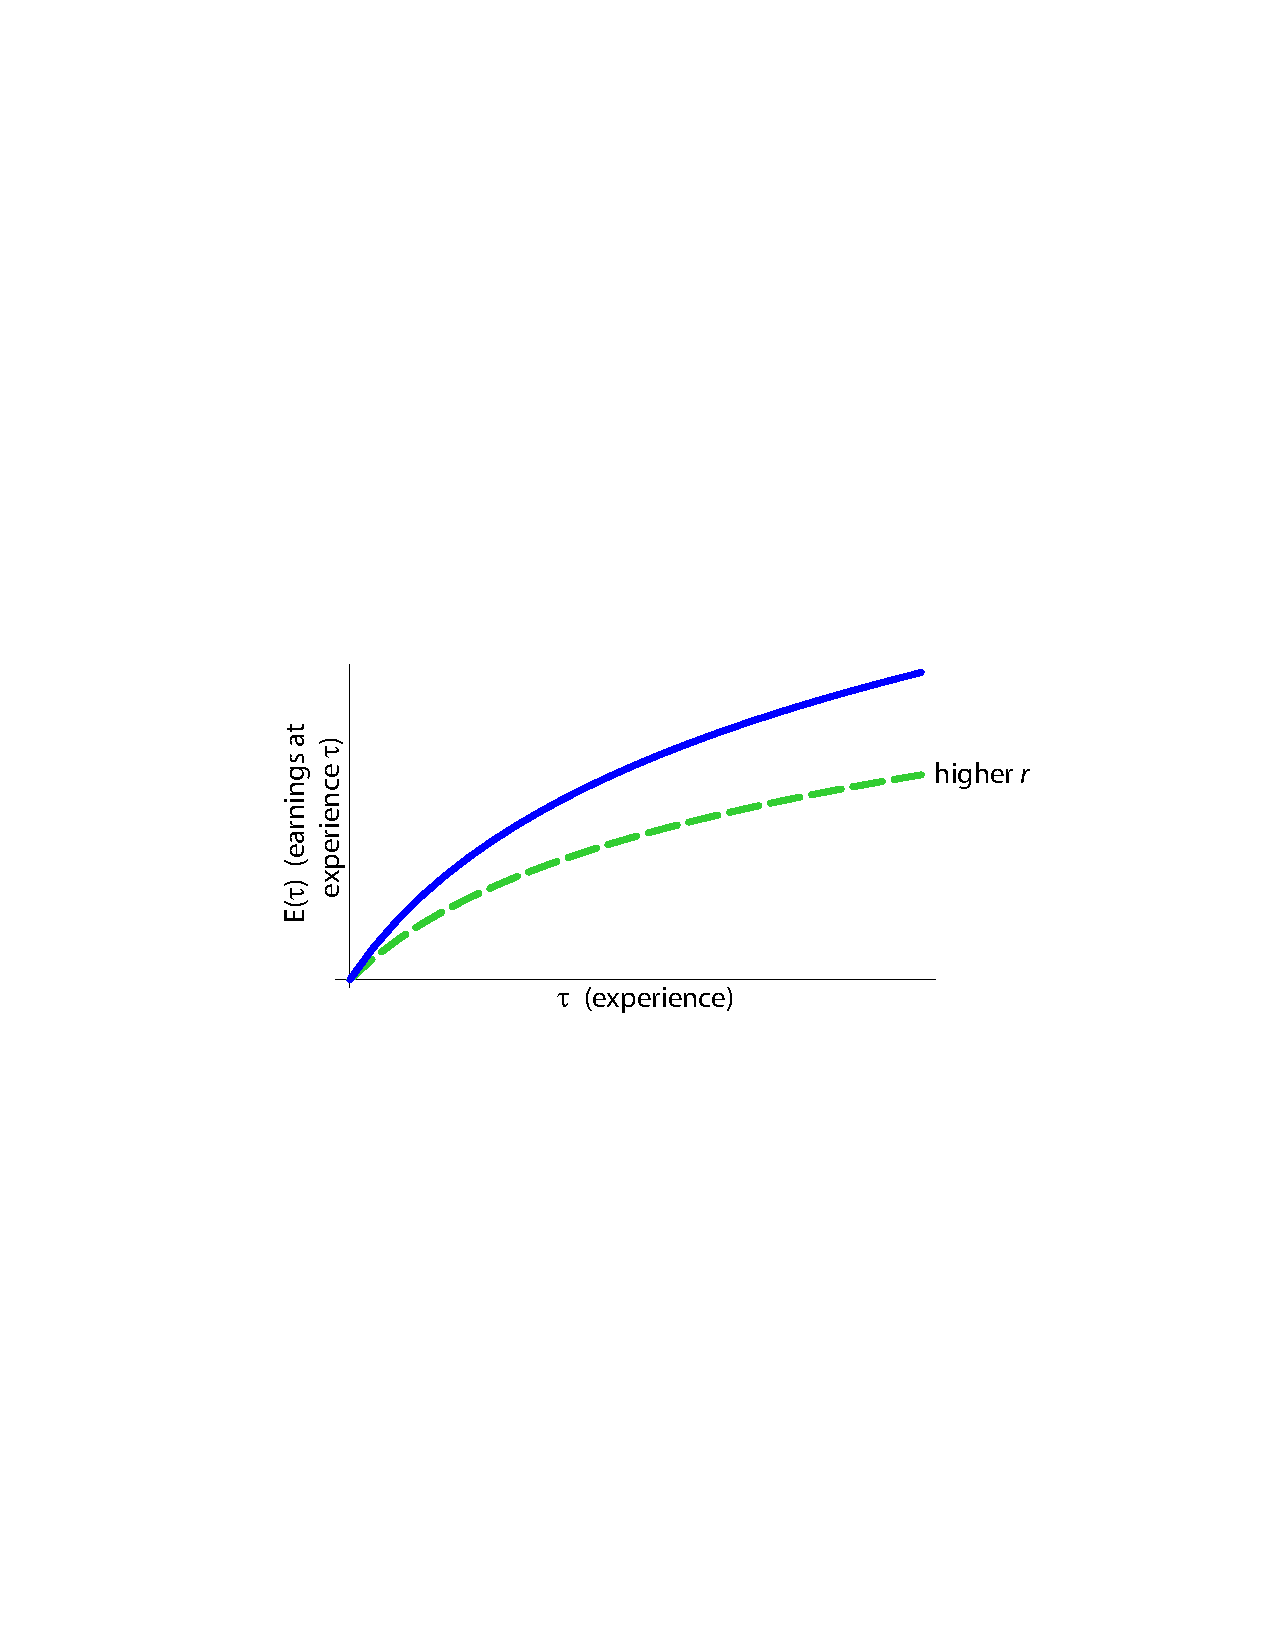
\includegraphics[width=3.5in, height=1.5in]{Figures/fig-earnings-growth.pdf}
\floatfoot{\begin{small}
Note:
\end{small}}
\end{figure}
\end{center}
 
\section{Generalized Ben-Porath Model}
Let us consider a generalization of the model in Section \ref{section:baseline} and allow for the law of motion of human capital to be
\begin{equation}
\dot{H} = A I^{\alpha} H^{\beta} - \sigma H \label{eq:lawhgen}.
\end{equation}

\indent This baseline Ben-Porath model is a particular case of this general formulation when $\alpha = \beta$. To simplify the analysis of the implications of this model we assume that there neither discounting nor depreciation, i.e. $r = \sigma = 0$. To ease notation we neglect the argument $t$ when possible. We analyze this model in finite horizon and follow the same notation as in Section \ref{section:baseline}. Thus, the agent's problem is to maximize
\begin{equation}
\max_{I(t)} \int _{0} ^{T} \left[ RH(t) \left(1 - I(t) \right) \right]dt
\end{equation}

\noindent subject to an initial condition for the stock of human capital, $H(0) = H_{0}$, and \eqref{eq:lawhgen}. The Hamiltonian of the problem is
\begin{equation}
\mathcal{H} = RH(t) \left(1 - I(t) \right) + \mu \left( A I^{\alpha} H^{\beta} \right)
\end{equation} 

where $\mu(t)$ defines the shadow price of human capital. The first order conditions are
\begin{eqnarray}
\frac{\partial \mathcal{H} (\cdot)}{\partial I(t)} = 0 &\Leftrightarrow& \mu A \alpha I^{\alpha - 1} H^{\beta} \geq RG \label{eq:focinvestmentgen} \\
\frac{\partial \mathcal{H} (\cdot)}{\partial H(t)} = - \dot{\mu(t)} &\Leftrightarrow& -R(1 - I) - \beta \mu A I^{\alpha} H^{\beta -1} \label{eq:focstockgen} \\ 
\frac{\partial \mathcal{H} (\cdot)}{\partial \mu(t)} = \dot{H} &\Leftrightarrow& \dot{H(t)} = F \left( I(t) H(t), D(t) \right) - \sigma D(t) \label{eq:focmotiongen} \\
\text{Transversality} &:& \lim_{t \rightarrow T} \mu(t) H(t) = 0 \label{eq:foctransversalitygen}
\end{eqnarray}

Importantly, these conditions are equivalent to the Mangasarian sufficient conditions for a global optimum if $\beta \leq 1$ \citep[see][]{mangasarian1966sufficient}.

\subsection{Specialization}
The specialization or schooling period when $I = 1$ happens if
\eqref{eq:focinvestmentgen} holds with strict inequality for $I=1$.
\begin{eqnarray}
\text{Conditions for Specialization :}
\begin{cases}
H > \left[ \frac{R}{\alpha A \mu} \right]^{\frac{1}{\beta - 1}}, & \beta > 1 \\
1 > \left[ \frac{R}{\alpha A \mu} \right]^{\frac{1}{\beta - 1}}, & \beta = 1 \\
H < \left[ \frac{R}{\alpha A \mu} \right]^{\frac{1}{\beta - 1}}, & \beta < 1. \\
\end{cases}
\end{eqnarray}

\noindent During this period \eqref{eq:focstockgen}, \eqref{eq:focmotiongen} become 
\begin{eqnarray}
\dot{\mu} &=& - \beta \mu A H^{\beta - 1} \label{eq:focstockgenspe} \\
\dot{H}  &=& A H^{\beta}. \label{eq:focmotiongenspe}\\
\end{eqnarray}

\indent We can solve for \eqref{eq:focmotiongenspe} and get
\begin{eqnarray}
H(t) =
\begin{cases}
c_{0} \exp^{At}, & \beta = 1 \\ 
\left( At + c_{1} \right)^{\frac{1}{1 - \beta}} (1 - \beta)^{\frac{1}{1 - \beta}}, & \beta \neq 1.

\end{cases}
\end{eqnarray}

\noindent The initial condition for the human capital stock leads to $c_{0} = \frac{H_{0}}{\exp^{1}} $ and $c_{1} = \frac{H_{0}^{1 - \beta}}{1-\beta}$ which implies that
\begin{eqnarray}
H(t)
\begin{cases}
H_{0} \exp^{At - 1}, & \beta = 1 \\
\left( At + \frac{H_{0}^{\frac{1}{1-\beta}}}{1-\beta} \right)^{\frac{1}{1 - \beta}} \left( 1 - \beta \right)^{\frac{1}{1-\beta}}, & \beta \neq 1. \label{eq:humanspe}
\end{cases}
\end{eqnarray}

\indent Also, we can solve \eqref{eq:focstockgenspe} and find that
\begin{eqnarray}
\mu(t) =
\begin{cases}
k_{0} \exp^{-At}, & \beta = 1 \\
\frac{k_{1}}{(At + c_{1})^{\frac{\beta}{1-\beta}}}, & \beta \neq 1 \label{eq:muspe}
\end{cases}
\end{eqnarray}

\noindent for which there is an exact solution given an initial condition $\mu(0) = \mu_{0}$. This is, we can find $k_{0}, k_{1}$ in \eqref{eq:muspe} provided $\mu_{0} > 0$ (it is a price). In particular, note that $k_{0} = \mu_{0} > 0$ and $k_{1} = \mu_{0} c_{1}^{\frac{\beta}{1-\beta}} > 0$ for $0<\beta<1$.\\
\indent Let $t^*$ denote the time when specialization ends. It must be true that, then, \eqref{eq:focinvestmentgen} holds with strict equality\footnote{typo in slide 18. All the time arguments in the first equation should be $t^*$.}
\begin{equation}
\mu(t^*) A \alpha H(t^*)^{\beta} = RH(t^*)
\end{equation}

\noindent which implies that 
\begin{equation}
t^* = \frac{1}{A} \left( \ln \left[ \frac{A\alpha}{R} + \ln k_{0} \right] \right)
\end{equation}

\noindent for $\beta = 1$. For $\beta \neq 1$, $t*$ solves
\begin{equation}
\frac{k_{1}}{ \left( At^* + c_{0} \right)^{\frac{\beta}{\beta-1}}} \frac{A \alpha}{R} = \left[ At^* \left( 1 - \beta \right)^{\frac{1}{1 - \beta}} + H_{0}^{1 - \beta} \left( 1 - \beta \right)^{\frac{\beta}{1 - \beta}} \right]^{1 - \beta}.
\end{equation}

\indent To wrap up the discussion we ask, if there is at least one period of specialization, how many periods of specialization there are. Consider two cases: (i) $\beta = 1$; (ii) $0 < \beta < 1$. In both cases, from \eqref{eq:muspe} we note that $\dot{mu(t)} < 0$. Importantly, $\mu(t)$ is the shadow price or value of human capital. Thus, $\dot{I(t)}$ and, if it exists, the period of specialization is unique.
 










